\documentclass[12pt]{book}
\usepackage{mathptm,times,color}
\usepackage[pdftex]{graphicx}
\usepackage{hyperref}
\usepackage{multirow}
\usepackage{longtable}
\usepackage{units}
\usepackage{fix-cm}
\usepackage{datetime}
\newdateformat{mydate}{\monthname[\THEMONTH] \THEYEAR}

\renewcommand{\bibname}{References}

%   dummy change to force revision update

%\usepackage{eso-pic}
%\usepackage{graphicx}
%\usepackage{color}
%\usepackage{type1cm}


%\makeatletter
%   \AddToShipoutPicture{%
%     \setlength{\@tempdimb}{.5\paperwidth}%
%    \setlength{\@tempdimc}{.5\paperheight}%
%   \setlength{\unitlength}{1pt}%
%  \put(\strip@pt\@tempdimb,\strip@pt\@tempdimc){%
%     \makebox(0,0){\rotatebox{45}{\textcolor[gray]{0.75}{\fontsize{8cm}{8cm}\selectfont{DRAFT}}}}}}
%\makeatother

\setlength{\textwidth}{6.5in}
\setlength{\textheight}{9.0in}
\setlength{\topmargin}{0.in}
\setlength{\headheight}{0.in}
\setlength{\headsep}{0.in}
\setlength{\parindent}{0.25in}
\setlength{\oddsidemargin}{0.0in}
\setlength{\evensidemargin}{0.0in}


%\includeonly{Overview_Chapter, SQA_Chapter, Structure_Chapter, Survey_Chapter, Experiment_Chapter, HGL_Chapter, Plume_Chapter, Species_Chapter, Pressure_Chapter, Heat_Flux_Chapter, Summary_Chapter}


\begin{document}

\bibliographystyle{unsrt}

\newcommand{\asqh}{$A_T/A\sqrt{h}$}
\newcommand{\degc}{$^{\circ}$C }
\newcommand{\degf}{$^{\circ}$F }
\newcommand{\brackets}[1]{ { \left( {#1} \right) } }
\newcommand{\dbydt}[1]{\frac{d {#1}}{dt}}
\newcommand{\ZQf}{\frac{Z}{Q_f^{2/5}}}
\newcommand{\dprime}{^{\prime \prime}}
\newcommand{\rH}{{\frac{r}{H}}}
\newcommand{\Dttwo}{{\frac{\Delta t}{2}}}

\newcommand{\superscript}[1]{\ensuremath{^{\textnormal{\scriptsize \hbox{#1}}}}}
\newcommand{\subscript}[1]{\ensuremath{_{\textnormal{\scriptsize \hbox{#1}}}}}


\newcommand{\dx}{\delta x}
\newcommand{\dy}{\delta y}
\newcommand{\dz}{\delta z}
\newcommand{\x}{x}
\newcommand{\y}{y}
\newcommand{\z}{z}
\newcommand{\dt}{\delta t}
\newcommand{\dn}{\delta n}
\newcommand{\cH}{{\cal H}}
\newcommand{\hu}{u}
\newcommand{\hv}{v}
\newcommand{\hw}{w}
\newcommand{\la}{\lambda}
%\newcommand{\bO}{\mbox{\boldmath $\Omega$}}
\newcommand{\bO}{{\Omega}}
\newcommand{\bo}{{\bf \omega}}
%\newcommand{\btau}{\mbox{\boldmath $\tau$}}
\newcommand{\btau}{{\bf \tau}}
\newcommand{\bdelta}{{\bf \delta}}
\newcommand{\sumym}{\sum (Y_i/W_i)}
\newcommand{\oW}{\overline{W}}
\newcommand{\om}{\omega}
\newcommand{\omx}{\omega_x}
\newcommand{\omy}{\omega_y}
\newcommand{\omz}{\omega_z}
\newcommand{\erf}{\hbox{erf}}
\newcommand{\bF}{{\bf F}}
\newcommand{\bof}{{\bf f}}
\newcommand{\bq}{{\bf q}}
\newcommand{\br}{{\bf r}}
\newcommand{\bu}{{\bf u}}
\newcommand{\bx}{{\bf x}}
\newcommand{\bk}{{\bf k}}
\newcommand{\bv}{{\bf v}}
\newcommand{\bg}{{\bf g}}
\newcommand{\bn}{{\bf n}}
\newcommand{\bS}{{\bf S}}
\newcommand{\dS}{d{\bf S}}
\newcommand{\bs}{{\bf s}}
\newcommand{\bI}{{\bf I}}
\newcommand{\hp}{{\cal H}}
\newcommand{\trho}{\tilde{\rho}}
\newcommand{\dph}{{\delta\phi}}
\newcommand{\dth}{{\delta\theta}}
\newcommand{\tp}{\tilde{p}}
\newcommand{\dQ}{\dot{Q}}
\newcommand{\dq}{\dot{q}}
\newcommand{\dm}{\dot{m}}
\newcommand{\ha}{\frac{1}{2}}
\newcommand{\ft}{\frac{4}{3}}
\newcommand{\ot}{\frac{1}{3}}
\newcommand{\fofi}{\frac{4}{5}}
\newcommand{\of}{\frac{1}{4}}
\newcommand{\twth}{\frac{2}{3}}
\newcommand{\R}{{\cal R}}
\newcommand{\be}{\begin{equation}}
\newcommand{\ee}{\end{equation}}
\newcommand{\RE}{\hbox{Re}}
\newcommand{\LE}{\hbox{Le}}
\newcommand{\PR}{\hbox{Pr}}
\newcommand{\PE}{\hbox{Pe}}
\newcommand{\NU}{\hbox{Nu}}
\newcommand{\SC}{\hbox{Sc}}
\newcommand{\SH}{\hbox{Sh}}
\newcommand{\WE}{\hbox{We}}
\newcommand{\COTWO}{{\tiny \hbox{CO}_2}}
\newcommand{\OTWO}{{\tiny \hbox{O}_2}}
\newcommand{\CO}{{\tiny \hbox{CO}}}
\newcommand{\HTWOO}{{\tiny \hbox{H}_2\hbox{O}}}
\newcommand{\NTWO}{{\tiny \hbox{N}_2}}
\newcommand{\F}{{\tiny \hbox{F}}}
\newcommand{\So}{{\tiny \hbox{S}}}
\newcommand{\M}{{\tiny \hbox{M}}}
\newcommand{\HCN}{{\tiny \hbox{HCN}}}
\newcommand{\HCl}{{\tiny \hbox{HCl}}}
\newcommand{\Hy}{{\tiny \hbox{H}}}
\newcommand{\C}{{\tiny \hbox{C}}}
\newcommand{\N}{{\tiny \hbox{N}}}
\newcommand{\Oh}{{\tiny \hbox{O}}}
\newcommand{\Cl}{{\tiny \hbox{Cl}}}

\frontmatter

\pagestyle{empty}

\begin{minipage}[t][9in][s]{6.5in}

\flushright{
    \fontsize{20}{24}\selectfont
    \bf{NIST Special Publication 1026r1\\
     October 2011 Revision\\}
     }

\vspace{1in}

\flushright{
  \fontsize{28}{33.6}\selectfont
   \bf{CFAST -- Consolidated Model of Fire \\
   Growth and Smoke Transport \\
   (Version 6) \\
   Technical Reference Guide \\}
   }

\vspace{.5in}


\flushright{
  \fontsize{14}{16.8}\selectfont
   Richard D. Peacock \\
   Glenn P. Forney \\
   Paul A. Reneke \\
}

\vspace{.5in}

\normalsize
\flushright{http://dx.doi.org/10.6028/NIST.SP.1026r1}

\vfill

\center{
\includegraphics[width=5.5in]{FIGURES/nistident}}

\end{minipage}

\newpage

\hspace{5in}

\newpage

\begin{minipage}[t][9in][s]{6.5in}

\flushright{
    \fontsize{20}{24}\selectfont
    \bf{NIST Special Publication 1026r1\\
     October 2011 Revision\\}
     }

\vspace{1in}

\flushright{
  \fontsize{28}{33.6}\selectfont
   \bf{CFAST -- Consolidated Model of Fire \\
   Growth and Smoke Transport \\
   (Version 6) \\
   Technical Reference Guide \\}
   }

\vspace{.5in}

\normalsize
\flushright{
Richard D. Peacock \\
Glenn P. Forney \\
Paul A. Reneke \\
{\em Fire Research Division} \\
{\em Engineering Laboratory}  \\
 }

 \vspace{.5in}
 
\flushright{http://dx.doi.org/10.6028/NIST.SP.1026r1}

\vspace{.25in}

\flushright{\mydate\today\\
SVN Repository~Revision: $Revision: 283 $}


%\vfill

\flushright{
\includegraphics[width=1in]{FIGURES/doc} }

\small
\flushright{U.S. Department of Commerce \\
{\em Rebecca M. Blank, Acting Secretary} \\
\vspace{\baselineskip}
National Institute of Standards and Technology \\
{\em Patrick D. Gallagher, Under Secretary for Standards and Technology and Director} }
\end{minipage}

\chapter{Disclaimer}

\pagestyle{plain}
\setcounter{page}{2}

The U. S. Department of Commerce makes no warranty, expressed or implied, to users of
CFAST and associated computer programs, and accepts no responsibility for its use.  Users of
CFAST assume sole responsibility under Federal law for determining the appropriateness of its
use in any particular application; for any conclusions drawn from the results of its use; and for
any actions taken or not taken as a result of analyses performed using these tools.
CFAST is intended for use only by those competent in the field of fire safety and is intended
only to supplement the informed judgment of a qualified user. The software package is a
computer model which may or may not have predictive value when applied to a specific set of
factual circumstances. Lack of accurate predictions by the model could lead to erroneous
conclusions with regard to fire safety. All results should be evaluated by an informed user.

\chapter{Intent and Use}

The algorithms, procedures, and computer programs described in this report constitute a
methodology for predicting some of the consequences resulting from a prescribed fire.  They
have been compiled from the best knowledge and understanding currently available, but have
important limitations that must be understood and considered by the user.  The program is
intended for use by persons competent in the field of fire safety and with some familiarity with
personal computers. It is intended as an aid in the fire safety decision-making process.

\chapter{Preface}

CFAST is a two-zone fire model used to calculate the evolving distribution of smoke, fire gases
and temperature throughout compartments of a constructed facility during a fire. In CFAST,
each compartment is divided into two gas layers.

The modeling equations used in CFAST take the mathematical form of an initial value problem
for a system of ordinary differential equations (ODEs). These equations are derived using the
conservation of mass, the conservation of energy (equivalently the first law of thermodynamics),
the ideal gas law and relations for density and internal energy. These equations predict as
functions of time quantities such as pressure, layer height and temperatures given the
accumulation of mass and enthalpy in the two layers. The CFAST model then consists of a set
of ODEs to compute the environment in each compartment and a collection of algorithms to
compute the mass and enthalpy source terms required by the ODEs.

In general, this document provides the technical documentation for CFAST along with
significant information on validation of the model. It follows the ASTM E1355 guide for model
assessment. The guide provides several areas of evaluation:

\begin{itemize}
\item Model and scenarios definition: CFAST is designed primarily to predict the
environment within compartmented structures which results from unwanted fires. These
can range from very small containment vessels, on the order of 1 m\superscript{3} to large spaces on
the order of 1000 m\superscript{3}. The appropriate size fire for a given application depends on the size
of the compartment being modeled. A range of such validation exercises is discussed in
chapter \ref{sec:validationsummary}.

\item Theoretical basis for the model: Details of the underlying theory, governing equations,
correlations, and organization used in the model are presented. The process of
development of the model is discussed with reference to a range of NIST memorandums,
published reports, and peer-reviewed journal articles on the model. In addition to overall
limitations of zone-fire modeling, limitations of the individual sub-models are discussed.

\item Mathematical and numerical robustness: CFAST has been subjected to extensive use
and review both internal to NIST and by users worldwide in a broad range of
applications. In addition to review within NIST independent of the model developers, the
model has been published in international peer-reviewed journals worldwide, and in
industry-standard handbooks referenced in specific consensus standards. Besides formal
internal and peer review, CFAST is subjected to continuous scrutiny because it is
available to the general public and is used internationally by those involved in fire safety
design and post-fire reconstruction.

\item Model sensitivity: Many of the outputs from the CFAST model are relatively insensitive
to uncertainty in the inputs for a broad range of scenarios. Not surprisingly, the heat
release rate is the most important variable because it provides the driving force for firedriven
flows. For CFAST, the heat release rate is prescribed by the user. Thus, careful
selection of the fire size is necessary for accurate predictions. Other variables related to
compartment geometry such as compartment height or vent sizes, while deemed
important for the model outputs, are typically more easily defined for specific design
scenarios than fire related inputs.

\item Model evaluation: The CFAST model has been subjected to extensive validation studies
by NIST and others. Although some differences between the model and the experiments
were evident in these studies, they are typically explained by limitations of the model and
uncertainty of the experiments. Most prominent in the studies reviewed was the overprediction
of gas temperature often attributed to uncertainty in soot production and
radiative fraction. Still, studies typically show predictions accurate within about 30 \%
of measurements for a range of scenarios. Like all predictive models, the best predictions
come with a clear understanding of the limitations of the model and of the inputs
provided to the calculations.

\end{itemize}

\chapter{Nomenclature}

\begin{center}
\begin{longtable}{p{1in}  p{5.5 in}}

 $A$ & area, m\superscript{2} \\
 $A_{slab}$ & cross-sectional area of vent slab in horizontal vent flow, m\superscript{2} \\
 $A_v$ & cross-sectional area of a vent, m\superscript{2} \\
 $C$ & vent constriction (or flow) coefficient, dimensionless \\
 $C_{LOL}$ & lower oxygen limit coefficient, fraction of the available fuel which can be burned with the available oxygen, dimensionless \\
 $C_T$ & constant from plume centerline temperature calculation, 9.115 \\
 $c_p$ & heat capacity of air at constant pressure, J/kg K \\
 $c_v$ & heat capacity of air at constant volume, J/kg K \\
 $D$ & fire diameter, m \\
 $D^*$ & characteristic fire diameter parameter, $\brackets{Q_f/\brackets{\rho_\infty c_p T_\infty \sqrt{g}}}^{2/5}$ \\
  & vent diameter, m \\
  $d_0$ & inlet ceiling jet depth in corridor flow, m \\
 $E_O$ & energy release per unit mass of oxygen consumed, J/kg \\
 $E_i$ & internal energy in layer $i$, W \\
 $F_{k-j}$ & configuration factor, fraction of radiation given off by surface $k$ intercepted by surface $j$, dimensionless \\
 $g$ & gravitational constant, 9.8 m/s\superscript{2} \\
 $h$ & convective heat transfer coefficient (W/m\superscript{2} K) \\
 $\dot{h}_i$ & rate of addition of enthalpy into layer $i$, J/s \\
 $\dot{h}_L$ & rate of addition of enthalpy into lower layer in a compartment, J/s \\
 $\dot{h}_U$ & rate of addition of enthalpy into upper layer in a compartment, J/s \\
 $H$ & height of a compartment, m \\
          & flame height, m \\
 $H_1$ & distance from fire source to target location in plume centerline temperature calculation, m \\
 $H_2$ & distance from virtual fire source to target location in plume centerline temperature calculation, m \\
 $H_c$ & heat of combustion of the fuel, J/kg \\
 $k$ & equivalent thermal conductivity of air, W/m K, with subscripts c,e and s \\
 $k$ & equilibrium coefficient for HCl transport and deposition \\
 $L$ & length of a compartment, m \\
  & characteristic length for radiation calculation, m \\
 $M_\F$ & molar mass of fuel, kg/mol \\
 $M_{\OTWO, \COTWO, ... \HCN, \So}$ & molar mass of oxygen, carbon dioxide, water, carbon monoxide, hydrochloric acid, hydrogen cyanide, and soot, kg/mol \\
 $m$ & mass, kg \\
 $\dot{m}_e$ & entrainment rate, kg/s \\
 $\dot{m}_{ex}$ & bi-directional vent flow in vertical flow vent, kg/s \\
 $\dot{m}_f$ & pyrolysis rate of the fire, kg/s \\
 $m_i$ & total mass in gas layer $i$, kg \\
 $\dot{m}_{io}$ & mass flow rate through a vent, kg/s \\
 $m_L$ & total mass in lower gas layer in a compartment, kg \\
 $\dot{m}_O$ & oxygen required for full combustion of available fuel, kg/s \\
 $\dot{m}_p$ & plume flow rate, kg/s \\
 $m_U$ & total mass in upper gas layer in a compartment, kg \\
 $P$ & pressure at floor level of a compartment, Pa \\
 $P_b$ & cross-vent differential pressure at the bottom of a vent flow slab in horizontal vent flow, Pa \\
 $P_t$ & cross-vent differential pressure at the top of a vent flow slab in horizontal vent flow, Pa \\
 $Q_{ceil}$ & average convective heat transfer from the ceiling jet to the ceiling surface, W \\
 $Q_f$ & total heat release rate of the fire, W \\
 $Q_{f,C}$ & heat release rate of the fire released as convective energy, W \\
 $Q_{f,eq}$ & effective heat release rate of a vent fire, kW \\
 $Q_{f,R}$ & heat release rate of the fire released as radiation, W \\
 $Q_{spray}$ & spread density of a sprinkler \\
 $Q_{I,1}^*$ & original fire strength for plume temperature calculation, dimensionless \\
 $Q_{I,2}^*$ & modified fire strength for plume temperature calculation when target location is in the upper layer, dimensionless \\
 $\Delta \hat{q}_k\dprime$ & net radiative flux at wall segment $k$ \\
 $q\dprime$ & heat flux, W/m\superscript{2} \\
 $R$ & universal gas conference, J/kg K \\
 $RTI$ & thermal characteristic response time index of a sprinkler or heat detector (m\superscript{1/2} s\superscript{1/2}) \\
 $r$ & radial distance from the fire, m \\
 $S$ & vent coefficient for vertical flow vents, dimensionless \\
 $T_\infty$ & ambient gas temperature in compartment well removed from a target, K \\
 $T_{amb}$ & ambient temperature, K \\
 $T_i$ & gas temperature of layer $i$, K \\
 $T_L$ & gas temperature of lower layer in a compartment, K \\
 $T_p$ & gas temperature in the plume, K \\
 $T_U$ & gas temperature of upper layer in a compartment, K \\
 $T_{0}$ & inlet gas temperature of the ceiling jet in corridor flow, K \\
 $T_1^*$ & calculated plume temperature at the transition between continuous flaming and intermittent flaming, K \\
 $T_2^*$ & calculated plume temperature at the transition intermittent flaming and the fire plume, K \\
 $t$ & time, s \\
 $V$ & total volume of a compartment, m\superscript{3} \\
 $V_L$ & total volume of lower layer in a compartment, m\superscript{3} \\
 $V_U$ & total volume of upper layer in a compartment, m\superscript{3} \\
 $V_i$ & volume of gas layer $i$, m\superscript{3} \\
 $v$ & velocity, m/s \\
 $v_0$ & inlet ceiling jet velocity in corridor flow, m/s \\
 $W$ & width of a compartment, m; wall thickness, m \\
 $Y_{LOL}$ & mass fraction of oxygen below which combustion will no longer occur, dimensionless \\
 $Y_{O_2}$ & mass fraction of oxygen in a gas layer, dimensionless \\
 $y_s$ &  soot yield, mass of soot produced by the fire per unit mass of fuel, kg/kg \\
 $Z_{I,1}$ & distance from fire source to the interface between upper and lower layers, m \\
 $Z_{I,2}$ & distance from virtual fire source to the interface between upper and lower layers, m \\
 $z$ & height above the base of the fire, m \\
 $z_{\nu}$ & height of the virtual origin of a vent fire, m \\
 $z_p$ & reduced height of the plume of a vent fire, m \\
 $z_0$ & height of the virtual origin of fire, m \\
 $z_1^*$ & height above the base of the fire at the transition between continuous flaming and intermittent flaming, m \\
 $z_2^*$ & height above the base of the fire at the transition intermittent flaming and the fire plume, m \\
  \\

 $\alpha$ & gas absorptance, dimensionless \\
  & thermal diffusivity in conduction (m\superscript{2}/s) \\
  $\beta$ & experimentally-determined constant in plume centerline temperature calculation, $\beta^2 = 0.913$ \\
 $\gamma$ & ratio of $c_p / c_v$, dimensionless \\
 $\Delta T$ & temperature rise, K \\
 $\epsilon$ & emissivity \\
 $\nu$ & stoichiometric coefficients for combustion reaction, dimensionless \\
            & kinematic viscosity, m\superscript{2}/s \\
 $\rho$ & density, kg/m\superscript{3} \\
 $\rho_\infty$ & density of gas well removed from a target, kg/m\superscript{3} \\
 $\rho_{cj}$ & density of the ceiling jet gas, kg/m\superscript{3}  \\
 $\rho_i$ & density of gas layer $i$, kg/m\superscript{3}  \\
 $\sigma$ & Stefan-Boltzman constant (5.67 x 10\superscript{-8} W/m\superscript{2}K\superscript{4}) \\
 $\tau$ & transmittance, dimensionless \\
 $\chi_C$ & fraction of the fire's heat release rate released as convective energy, dimensionless \\
 $\chi_R$ & fraction of the fire's heat release rate released as radiation, dimensionless \\
 $\xi$ & ratio of upper layer gas temperature to lower layer gas temperature, dimensionless \\

\end{longtable}

\end{center}

\chapter{Acknowledgments}

\label{acksection}

Continuing support for CFAST is via internal funding at NIST. In addition, support is provided by other agencies of the U.S. Federal Government, most notably the Nuclear Regulatory Commission Office of Research and the U.S. Department of Energy. The U.S. NRC Office of Research has funded key validation experiments, the preparation of the CFAST manuals, and the continuing development of sub-models that are of importance in the area of nuclear power plant safety. Special thanks to Mark Salley, David Stroup, and Jason Dreisbach for their efforts and support. Support to refine the software development and quality assurance process for CFAST has been provided by the U.S. Department of Energy (DOE). The assistance of Subir Sen and Debra Sparkman in understanding DOE software quality assurance programs and the application of the process to CFAST is gratefully acknowledged.  

Doug Carpenter, Combustion Sciences and Engineering, has contributed numerous corrections, clarifications, and updates to the guides and the model through his detailed review of the model and documentation. Allan Coutts, Washington Safety Management Solutions, provided insight into the application of fire models to nuclear safety applications and detailed review of the CFAST document updates for DOE.


\tableofcontents

\listoffigures

\listoftables

\mainmatter

\chapter{Overview}

This chapter provides a general description of the Consolidated Fire and Smoke Transport (CFAST) model following the guidance in ASTM~E1355~\cite{ASTM:E1355}.

\section{Model Documentation}

\subsection{Name and Version of the Model}

The name of the model is the Consolidated Fire Growth and Smoke Transport Model or CFAST. The first public release was version 1.0 in June, 1990. This version was restructured from FAST~\cite{Models:FAST} to incorporate the ``lessons learned'' from the zone model CCFM developed by Cooper and Forney~\cite{Models:CCFM}. Version~2 was released as a component of Hazard~1.2 in 1994~\cite{Models:HAZARDI, Models:HAZARDI_12}. The first of the 3.x series was released in 1995 and included a vertical flame spread algorithm, ceiling jets and non-uniform heat loss to the ceiling, spot targets, and heating and burning of multiple objects (ignition by flux, temperature or time) in addition to multiple prescribed fires. As it evolved over the next five years, version~3 included smoke and heat detectors, suppression through heat release reduction, better characterization of flow through doors and windows, vertical heat conduction through ceiling/floor boundaries, and non-rectangular compartments. In 2000, version~4 was released and included horizontal heat conduction through walls, and horizontal smoke flow in corridors. Version~5 improved the combustion chemistry. Version 6, released in July, 2005, incorporates a more consistent implementation of vents, fire objects and event processing and includes a graphical user interface which substantially improves its usability.

\subsection{Type of Model}

CFAST is a two-zone fire model that predicts the thermal environment within compartmented structures resulting from a fire. Each compartment is divided into an upper and lower gas layer. The fire drives combustion products from the lower to the upper layer via the plume. The temperature within each layer is uniform, and its evolution in time is described by a set of ordinary differential equations.

\subsection{Model Developers}

CFAST was developed and is maintained primarily by the Fire Research Division of the National Institute of Standards and Technology. The developers are Walter Jones, Richard Peacock, Glenn Forney, Rebecca Portier, Paul Reneke, and John Hoover \footnote{Naval Research Laboratory, Washington, DC 20375.}.

There have been contributions through research and published papers at Worcester Polytechnic Institute, University of California at Berkeley, VTT of Finland and CITCM of France. An important guide to development of the model has been from many people around the world who have provided ideas, suggestions, comments, detailed questions, opinions on what should happen in particular scenarios, what physics and chemistry are needed and what types of problems must be addressed by such a model in order to be useful for real world applications.

\subsection{Relevant Publications}

To accompany the model and simplify its use, NIST has developed this Technical Reference Guide \cite{CFAST_Tech_Guide_6}, a User's Guide \cite{CFAST_Users_Guide_6} and a Software and Validation Guide \cite{CFAST_Valid_Guide_6}.  The Technical Reference Guide describes the underlying physical principles and summarizes sensitivity analysis, model validation, and model limitations consistent with ASTM E 1355 \cite{ASTM:E1355}.  The User�s Guide describes how to use the model.

The U.S. Nuclear Regulatory Commission has published a verification and validation study of five selected fire models commonly used in support of risk-informed and performance-based fire protection at nuclear power plants \cite{NRCNUREG1824_CFAST}. In addition to an extensive study of the CFAST model, the report compares the output of several other models ranging from simple hand calculations to more complex CFD codes such as the Fire Dynamics Simulator (FDS) developed by NIST.

There are documents available (http://cfast.nist.gov) that are applicable to versions 2, 3, 5 as well as 6 of both the model and user interface.

\subsection{Governing Equations and Assumptions}

For CFAST, as for most zone fire models, the equations solved are for conservation of mass and energy. The momentum equation is not solved explicitly, except for use of the Bernoulli equation for the flow velocity at vents. Based on an integration over the volume of an element, these equations are solved as ordinary differential equations.

There are two assumptions which reduce the computation time dramatically. The first is that relatively few zones or elements per compartment is sufficient to model the physical situation. The second assumption is to close the set of equations without using the momentum equation in the compartment interiors. This simplification eliminates acoustic waves. Though this prevents one from calculating gravity waves in compartments (or between compartments), coupled with only a few elements per compartment allows for a prediction in a large and complex space very quickly.



\subsection{Input Data Required to Run the Model}

All of the data required to run the CFAST model reside in a primary data file, which the user creates.  Some instances may require databases of information on objects, thermophysical properties of boundaries, and sample prescribed fire descriptions.  In general, the data files contain the following information:
\begin{itemize}
\item compartment dimensions (height, width, length)
\item construction materials of the compartment (e.g., concrete, gypsum)
\item material properties (e.g., thermal conductivity, specific heat, density, thickness, heat of combustion)
\item dimensions and positions of horizontal and vertical flow openings such as doors, windows, and vents
\item mechanical ventilation specifications
\item fire properties (e.g., heat release rate, lower oxygen limit, and species production rates as a function of time)
\item sprinkler and detector specifications
\item positions, sizes, and characteristics of targets
\end{itemize}
The input files are provided for the validation exercises described in the Validation Guide~\cite{CFAST_Valid_Guide_6}. These examples range from simple one-compartment simulations to a large multi-story hotel scenario that includes an elevator shaft and stairwell pressurization. A complete description of the input parameters required by CFAST can be found in the CFAST User's Guide \cite{CFAST_Users_Guide_6}. Some of these parameters have default values included in the model, which are intended to be representative for a range of fire scenarios.

\subsection{Property Data}

Any simulation of a real fire scenario involves prescribing material properties for the walls,
floor, ceiling, and furnishings. CFAST treats all of these materials as homogeneous solids, thus
the physical parameters for many real objects can only be viewed as approximations to the actual
properties. Describing these materials in the input data file is a challenging task for the model
user. Thermal properties for the most common barrier materials used in construction, e.g.
gypsum wall board, are included in a database, thermal.df, included with the model. These
properties come directly from handbook values for typical materials \cite{Incorpera:1981}.

\subsection{Model Results}

The output of CFAST are the sensible variables that are needed for assessing the environment in a building subjected to a fire. Once the simulation is complete, CFAST produces an output file containing all of the solution variables.  Typical outputs include (but are not limited to) the following:
\begin{itemize}
\item environmental conditions in the room (such as hot gas layer temperature; plume centerline temperature; oxygen and smoke concentration; and ceiling, wall, and floor temperatures)
\item heat transfer-related outputs to walls and targets (such as incident convective, radiated, and total heat fluxes)
\item fire intensity and flame height
\item flow velocities through vents and openings
\item detector and sprinkler activation times
\end{itemize}
There is more extensive discussion of the output in chapter 6 of this technical reference manual and the user's guide. The output is always in the metric system of units.

\subsection{Uses and Limitations of the Model} \label{sec:limitssummary}

CFAST has been developed for use in solving practical fire problems in fire protection engineering.  It is intended for use in system modeling of building and building components.  A priori prediction of flame spread or fire growth on objects is not modeled. Rather, the consequences of a specified fire is estimated. It is not intended for detailed study of flow within a compartment, such as is needed for smoke detector siting.  It includes the activation of sprinklers and fire suppression by water droplets.

The most extensive use of the model is in fire and smoke spread in complex buildings.  The efficiency and computational speed are inherent in the few computation cells needed for a zone model implementation.  The use is for design and reconstruction of time-lines for fire and smoke spread in residential, commercial, and industrial fire applications.  Some applications of the model have been for design of smoke control systems.

\begin{itemize}
\item Compartments:  CFAST is generally limited to situations where the compartment volumes are strongly stratified.  However, in order to facilitate the use of the model for preliminary estimates when a more sophisticated calculation is ultimately needed, there are algorithms for corridor flow, smoke detector activation, and detailed heat conduction through solid boundaries.  This model does provide for non-rectangular compartments, although the application is intended to be limited to relatively simple spaces.  There is no intent to include complex geometries where a complex flow field is a driving force.  For these applications, computational fluid dynamics (CFD) models are appropriate.

\item Gas Layers:  There are also limitations inherent in the assumption of stratification of the gas layers.  The zone model concept, by definition, implies a sharp boundary between the upper and lower layers, whereas in reality, the transition is typically over about 10~\% of the height of the compartment and can be larger in weakly stratified flow.  For example, a burning cigarette in a normal room is not within the purview of a zone model.  While it is possible to make predictions within 5~\% of the actual temperatures of the gas layers, this is not the optimum use of the model.  It is more properly used to make estimates of fire spread (not flame spread), smoke detection and contamination, and life safety calculations.

\item Heat Release Rate:  CFAST does not predict fire growth on burning objects. Heat release rate is specified by the user for one or more fire objects. The model does include the ability to limit the specified burning based on available oxygen. There are also limitations inherent in the assumptions used in application of the empirical models.  As a general guideline, the heat release should not exceed about 1 MW/m$^3$.  This is a limitation on the numerical routines attributable to the coupling between gas flow and heat transfer through boundaries (conduction, convection, and radiation).  The inherent two-layer assumption is likely to break down well before this limit is reached.

\item Radiation:  Because the model includes a sophisticated radiation model and ventilation algorithms, it has further use for studying building contamination through the ventilation system, as well as the stack effect and the effect of wind on air circulation in buildings.  Radiation from fires is modeled with a simple point source approximation.  This limits the accuracy of the model near fire sources. Calculation of radiative exchange between compartments is not modeled.

\item Ventilation and Leakage:  In a single compartment, the ratio of the volume of the compartment to the area of vents connecting the compartment to another should not exceed roughly 2 m.  This is a limitation on the plug flow assumption for vents.  A more important limitation arises from the uncertainty in the scenario specification.  For example, leakage in buildings is significant, and this affects flow calculations especially when wind is present and for tall buildings.  These effects can overwhelm limitations on accuracy of the implementation of the vent flow model.  The overall accuracy of the model is closely tied to the specificity, care, and completeness with which the data are provided.

\item Thermal Properties:  The accuracy of the model predictions is limited by how well the user can specify the thermophysical properties.  For example, the fraction of fuel which ends up as soot has an important effect on the radiation absorption of the gas layer and, therefore, the relative convective versus radiative heating of the layers and walls, which in turn affects the buoyancy and flow.  There is a higher level of uncertainty of the predictions if the properties of real materials and real fuels are unknown or difficult to obtain, or the physical processes of combustion, radiation, and heat transfer are more complicated than their mathematical representations in CFAST.
\end{itemize}

User feedback indicates that using CFAST to predict the transport of heat and combustion
products from a prescribed fire is straightforward, easily and quickly accomplished, and the
results are within expectations. Any user of a computer based (numerical) model must be aware
of the assumptions and approximations being employed. Except for those few materials supplied
in the property databases, the user must supply the thermal properties of the materials, and then
assess the performance of the model compared with experiments to ensure that the model is valid
for a specific application. Only then can the model be expected to predict the outcome of fire
scenarios that are similar to those that have actually been tested.

In addition, there are specific limitations and assumptions made in the development of the algorithms.  These are detailed in the discussion of each of these sub-models:

In addition, there are specific limitations and assumptions made in the development of the
algorithms. These are detailed in the discussion of each of these sub-models:

\begin{itemize}
\item section \ref{sec:ZoneModelAssumptions} on zone model assumptions,
\item section \ref{sec:TheFire} on prescribed fires,
\item section \ref{sec:firemassbalance} on the relationship between fires and mass balance,
\item section \ref{sec:plumelimits} on the plume entrainment model,
\item section \ref{sec:corridorflow} on the assumptions made for corridor flow correlations,
\item section \ref{sec:Radiation} on the assumptions made for radiation heat transfer,
\item section \ref{sec:suppression} on the suppression model, and
\item section \ref{HClDeposition} on HCl deposition.
\end{itemize}

\section{Scenarios for which the Model is Evaluated in this Document}

CFAST is used for a wide range of buildings of interest, from glove-box size compartments, to complex hotels to the vehicle assembly building at Cape Canaveral. The intended use of ASTM~E1355~\cite{ASTM:E1355} is to validate a specific scenario of interest so that the model can be used for scenarios similar to the chosen scenario. The intent of this document, however, is to cover a much wider range of scenarios which encompass the range of acceptable use of the model. Thus, this section provides a description of this broader range of scenarios as discussed in this technical reference guide rather than a single, specific scenario of interest for a validation exercise.

\subsection{Description of Scenarios of Interest}

CFAST is designed primarily to predict the environment within compartmented structures which results from unwanted fires. These can range from very small containment vessels, on the order of 1 m\superscript{3} to large spaces on the order of 1000 m\superscript{3}. As discussed in the section on limitations and use (see section \ref{sec:limitssummary}), the appropriate size fire depends on the size of the compartment being modeled. A range of such validation exercises is discussed in chapter \ref{sec:validationsummary}.

\subsection{List of Quantities Predicted by the Model}

CFAST provides a prediction of the plume centerline, gas layer, and boundary temperatures, target temperatures, species concentration (including soot volume fraction), layer height, fire size and flame length, floor pressure, flow and fire size at vents, and heat flux (both radiative and convective). There is a more extensive discussion of the output in the CFAST user's guide.

\subsection{Degree of Accuracy Required for Each Output Quantity}

The degree of  accuracy for each output variable  required by the user is  highly  dependent on  the  technical  issues  associated with  the analysis.  The user  must ask: How accurate does  the analysis have to be  to  answer  the  technical  question posed?  Thus,  a  generalized definition of the  accuracy required for each quantity  with no regard as  to the specifics  of a  particular analysis  is not  practical and would be limited in its usefulness.

Returning   to    the   earlier   definitions    of   ``design''   and ``reconstruction,'' fire scenarios, design applications  typically are  more accurate because the heat release rate is prescribed rather than predicted, and the    initial    and    boundary    conditions   are    far    better characterized. Mathematically, a design calculation is an example of a ``well-posed''  problem  in  which   the  solution  of  the  governing equations is  advanced in  time starting from  a known set  of initial conditions and constrained by a known set of boundary conditions.  The accuracy of the results is a function of the fidelity of the numerical solution, which is  largely dependent on the quality of the model inputs.

A reconstruction is an example of an ``ill-posed'' problem because the outcome  is known  whereas  the initial  and  boundary conditions  are not. There is  no single, unique solution to the  problem. Rather, it is possible to simulate numerous fires that produce the given outcome. There is no right or wrong answer, but rather a small set of plausible fire scenarios that are  consistent with the collected evidence and physical laws incorporated into the model. These simulations are then used to demonstrate why the fire behaved as it did  based on the current understanding of fire physics  incorporated in  the model.  Most  often, the  result of  the
analysis is only  qualitative. If there is any  quantification at all, it could be in the time to reach critical events, like a roof collapse or room flashover.

The CFAST validation guide \cite{CFAST_Valid_Guide_6} includes efforts to date involving well-characterized geometries and prescribed fires. These studies show that  CFAST predictions vary from being within experimental   uncertainty  to  being   about  30~\%   different  than measurements of temperature, heat flux, gas concentration, {\em etc} (see, for example, reference \cite{NRCNUREG1824_CFAST}). In general, this is adequate for its intended uses which are life-safety calculations and estimation of the environment to which building elements are subjected in a fire environment. Applied design margins are typically larger than this level of accuracy and may be
appropriate to insure an adequate factor of safety.


\section{Review of the Theoretical Development of the Model}

Details of the software quality assurance process for CFAST is included in the Software and Model Evaluation Guide~\cite{CFAST_Valid_Guide_6}. A brief summary is provided here. 

CFAST has been subjected to independent review in two ways, internal and external. First, all documents issued by the National Institute of Standards and Technology receive three levels of internal review by members of the staff not involved in the preparation of the report or underlying research. The theoretical basis of CFAST is presented in this document, and is subject to internal review by staff members who are not active participants in the development of the model, but who are members of the Fire Research Division and are considered experts in the fields of fire and combustion. Externally, the theoretical basis for the model has been published in peer reviewed journals~\cite{Jones:1993a, Jones:1985, Jones:1984} and conference proceedings~\cite{Jones:1991}. In addition, CFAST is used worldwide by fire protection engineering firms who review the technical details of the model related to their particular application. Some of these firms also publish in the open literature reports documenting internal efforts to validate the model for a particular use. Many of these studies are discussed in more detail in the present document.

In addition to the formal review, procedures were in place during the development of CFAST to assure the quality of the model.  These procedures included several components:
\begin{itemize}
\item Review of proposed changes to the code by at least two others involved in the development process to insure that a proposed change was consistent with the rest of the CFAST code and was implemented correctly. These reviews, while informal in nature, provided a comprehensive review of the changes to the model during its development.  
\item In addition to the normal NIST document review process, the CFAST software was circulated internally to Fire Research Division Staff to allow interested staff members to test the model.
\item For each major release of CFAST, NIST has maintained a history of the source code which goes back to March 1989.  While it is not practical to reconstruct the programs for each release for use with modern software tools and computer operating systems, the source code history allows the developers to examine what changes were made at each release point. This provides detailed documentation of the history of model development and is often useful to understand the impact of changes to sub-models over the development of the model.
\item Once a release of CFAST was approved by NIST, it was announced with a letter to model users which provided a summary of model changes and available documentation.  In essence, these were a condensation of the internal memorandums, without details or printout of specific code changes.  These memorandums provide documentation of the history of the model development.
\end{itemize}
Finally, CFAST has been reviewed and included in industry-standard handbooks such as the SFPE Handbook \cite{Walton:2003} and referenced in specific standards, including NFPA~805 \cite{NFPA805:2004} and NFPA~551 \cite{NFPA551:2004}.

\subsection{Assessment of the Completeness of Documentation}

There are three primary documents on CFAST, this Technical Reference Guide, the User?s Guide \cite{CFAST_Users_Guide_6}, and the Software Development and Model Evaluation Guide \cite{CFAST_Valid_Guide_6}.  This document is the Technical Reference Guide and provides documentation of the governing equations, assumptions, and approximations of the various submodels. It also includes a summary description of the model structure, and numerics.  The Model User?s Guide includes a description of the model input data requirements and model results. The Software Development and Model Evaluation Guide describes the software quality assurance process used in the development and maintenance of the model and includes an extensive discussion of the validation of the model.

The extensive formal review process for all NIST publications in part insures the quality of the CFAST Guides. In addition, the model developers routinely receive feedback from users on the completeness of the documentation and add clarifications when needed. It is estimated that there are several thousand users of CFAST. Before new versions of the model are released, there is a ``beta test'' period in which the users test the new version using the updated documentation. This process is similar, although less formal, to that which most computer software programs undergo. Training courses for use of the model in fire hazard analysis have been developed from the model documentation and presented at training courses worldwide \cite{Barnett:1990}.

\subsection{Assessment of Justification of Approaches and Assumptions}

The technical approach and assumptions of the model have been presented in the peer reviewed scientific literature and at technical conferences. Also, all documents released by NIST are required to go through an internal editorial review and approval process. This process is designed to ensure compliance with the technical requirements, policy, and editorial quality required by NIST. The technical review includes a critical evaluation of the technical content and methodology, statistical treatment of data, uncertainty analysis, use of appropriate reference data and units, and bibliographic references. CFAST manuals are always first reviewed by a member of the Fire Research Division, then by the immediate supervisor of the author of the document, then by the chief of the Fire Research Division, and finally by a reader from outside the division. Both the immediate supervisor and the division chief are technical experts in the field. Once the document has been reviewed, it is then brought before the Editorial Review Board (ERB), a body of representatives from all the NIST laboratories. At least one reader is designated by the Board for each document that it accepts for review. This last reader is selected based on technical competence and impartiality. The reader is usually from outside the division producing the document and is responsible for checking that the document conforms with NIST policy on units, uncertainty and scope. This reader does not need to be a technical expert in fire or combustion.

Besides formal internal and peer review, CFAST is subjected to continuous scrutiny because it is available to the general public and is used internationally by those involved in fire safety design and postfire reconstruction. The source code for CFAST is also released publicly, and has been used at various universities worldwide, both in the classroom as a teaching tool as well as for research. As a result, flaws in the theoretical development and the computer program itself have been identified and fixed. The user base continues to serve as a means to evaluate the model, which is as important to its development as the formal internal and external peer review processes.

\subsection{Assessment of Constants and Default Values}

A comprehensive assessment of the numerical parameters (such as default time step or solution convergence criteria) and physical parameters (such as empirical constants for convective heat transfer or plume entrainment) used in CFAST is not available in one document. Instead, specific parameters have been tested in various verification and validation studies performed at NIST and elsewhere. Numerical parameters are described in this Technical Reference Guide and are subject to the internal review process at NIST, but many physical parameters are extracted from the literature and do not undergo a formal review. In addition, default values for the various model inputs have been specifically reviewed by a professional fire protection engineering university professor to insure appropriate default values and suggested limits for the various input values. The model user is expected to assess the appropriateness of default values provided by CFAST and make changes to the default values if need be.

\subsection{Summary of Model Validation} \label{sec:validationsummary}

CFAST has been subjected to extensive validation studies by NIST and others.  There are two ways of comparing predictive capability with actual events. The first is simply graphing the time series curves of model results with measured values of variables such as temperature. Another approach is to consider the time to critical conditions such as flashover. Making such direct comparisons between theory and experiment provides a sense of whether predictions are reasonable. This chapter provides a review of CFAST validation efforts by NIST and others to better understand the quality of the predictions by the model.

Some of the work has been  performed at NIST, some by its grantees and some by engineering firms using the model.  Because each organization has its  own reasons for  validating the model, the  referenced papers and reports do not follow any particular guidelines. Some of the works only provide  a qualitative assessment  of the model,  concluding that the  model  agreement with  a  particular  experiment  is ``good''  or ``reasonable.'' Sometimes, the conclusion is that the model works well in certain cases, not as well in others. These studies are included in the survey because the references  are useful to other model users who may have a similar application  and are interested in qualitative assessment. It is important to note  that some of the papers point out flaws in early releases of CFAST that have been corrected or improved in more recent  releases. Some of  the issues raised, however,  are still subjects of  active research. Continued updates for CFAST  are greatly influenced  by   the  feedback   provided  by  users,   often  through publication of validation efforts.


A true validation of a model would involve proper statistical treatment of all the inputs and outputs of the model with appropriate experimental data to allow comparisons over the full range of the model. Thus, the comparisons of the differences between model predictions and experimental data discussed here are intentionally simple and vary from test to test and from variable to variable due to the changing nature of the tests and typical use of different variables. Table \ref{tab:Summary_Relative_Diffs} summarizes the Validation comparisons included for the current version of the model detailed in the Software Development and Experimental Evaluation Guide for CFAST \cite{CFAST_Valid_Guide_6}.

\begin{table}

\label{tab:Summary_Relative_Diffs}

\IfFileExists{../Validation_Guide/FIGURES/ScatterPlots/validation_statistics.tex}{\begin{center}
\begin{longtable}{|c|c|c|c|c|c|}
\hline
Quantity & Number of & Number of & $2\widetilde{\sigma}_E$ & $2\widetilde{\sigma}_M$ & Bias \\
         & Datasets  & Points    &                         &                         &      \\ \hline \hline
\endfirsthead
\hline
Quantity & Number of & Number of & $2\widetilde{\sigma}_E$ & $2\widetilde{\sigma}_M$ & Bias \\
         & Datasets  & Points    &                         &                         &      \\ \hline \hline
\endhead
HGL Temperature & 11 & 219 & 0.14 & 0.48 & 1.14 \\ \hline
HGL Temperature: Forced Ventilation & 7 & 91 & 0.14 & 0.39 & 1.25 \\ \hline
HGL Temperature: Natural Ventilation & 8 & 104 & 0.14 & 0.51 & 1.11 \\ \hline
HGL Temperature: No Ventilation & 3 & 22 & 0.14 & 0.69 & 1.32 \\ \hline
HGL Depth & 7 & 53 & 0.13 & 0.45 & 0.98 \\ \hline
Ceiling Jet Temperature & 6 & 208 & 0.10 & 0.44 & 1.23 \\ \hline
Plume Temperature & 4 & 51 & 0.14 & 0.42 & 1.17 \\ \hline
Oxygen Concentration & 6 & 40 & 0.09 & 0.61 & 1.04 \\ \hline
Carbon Dioxide Concentration & 5 & 31 & 0.09 & 0.49 & 0.85 \\ \hline
Smoke Concentration & 1 & 15 & 0.33 & 1.51 & 3.78 \\ \hline
Compartment Over-Pressure & 1 & 9 & 0.40 & 0.84 & 1.30 \\ \hline
Open Compartment Over-Pressure & 2 & 8 & 0.40 & 0.79 & 1.47 \\ \hline
Target Heat Flux & 1 & 100 & 0.20 & 1.30 & 1.01 \\ \hline
Wall Heat Flux & 6 & 121 & 0.20 & 0.75 & 1.21 \\ \hline
Target Temperature & 2 & 73 & 0.14 & 1.37 & 1.44 \\ \hline
Wall Temperature & 5 & 122 & 0.14 & 0.94 & 1.10 \\ \hline
Smoke Alarm Activations & 7 & 125 & 0.33 & 0.98 & 1.05 \\ \hline
Sprinkler Activation Time & 2 & 68 & 0.20 & 0.52 & 0.84 \\ \hline
\end{longtable}
\end{center}
}{\typeout{Error: Missing file FIGURES/ScatterPlots/validation_statistics.tex}}

\end{table}

Four of the quantities were seen to require additional care when using the model to evaluate the given quantity.  This typically indicates limitations in the use of the model.  A few notes on the comparisons are appropriate:

\begin{itemize}
\item CFAST typically predicts plume temperature near to experimental uncertainty, but tends to under-predict temperatures nearer to the fire source and over-predict temperatures farther away.
\item CFAST typically over-predicts smoke concentration.  Predicted concentrations for open-door tests are within experimental uncertainties, but those for closed-door tests are far higher.
\item With exceptions, CFAST predicts cable surface temperatures within experimental uncertainties.  Total heat flux to targets is typically predicted to within about 30~\%, and often under-predicted.  Radiative heat flux to targets is typically over-predicted compared to experimental measurements, with higher relative difference values for closed-door tests.  Care should be taken in predicting localized conditions (such as target temperature and heat flux) because of inherent limitations in all zone fire models.
\item Predictions of compartment surface temperature and heat flux are typically within 10~\% to 30~\%.  Generally, CFAST over-predicts the far-field fluxes and temperatures and under-predicts the near-field measurements.  This is consistent with the single representative layer temperature assumed by zone fire models.
\end{itemize}

CFAST predictions in this validation study were consistent with numerous earlier studies, which show that the use of the model is appropriate in a range of fire scenarios.  The CFAST model has been subjected to extensive evaluation studies by NIST and others.  Although differences between the model and the experiments were evident in these studies, most differences can be explained by limitations of the model as well as of the experiments.  Like all predictive models, the best predictions come with a clear understanding of the limitations of the model and the inputs provided to perform the calculations.




\chapter{Model and Scenario Definition}

Sufficient documentation of calculation models is necessary to assess the adequacy of the
scientific and technical basis of the model and the accuracy of the computational procedures for
scenarios of interest. In addition, adequate documentation will help prevent the unintentional
misuse of the model. The documentation in this document follows the guidelines in ASTM
E1355-04 \cite{ASTM:E1355}.

\section{Model Documentation}

\subsection{Name and Version of the Model}

The name of the model is the Consolidated Fire Growth and Smoke Transport Model or CFAST.
The first public release was version 1.0 in June of 1990. This version was restructured from
FAST \cite{Models:FAST} to incorporate the "lessons learned" from the zone model CCFM developed by Cooper
and Forney [\cite{Models:CCFM}, namely that modification is easier and more robust if the components such as the
physical routines are separated from the solver. chapter 4 (Mathematical and Numerical
Robustness) discusses this in more detail. Version 2 was released as a component of Hazard 1.2
in 1994 \cite{Models:HAZARDI, Models:HAZARDI_12}. The first of the 3.x series was released in 1995 and included a vertical flame spread
algorithm, ceiling jets and nonuniform heat loss to the ceiling, spot targets, and heating and
burning of multiple objects (ignition by flux, temperature or time) in addition to multiple
prescribed fires. As it evolved over the next five years, version 3 included smoke and heat
detectors, suppression through heat release reduction, better characterization of flow through
doors and windows, vertical heat conduction through ceiling/floor boundaries, and
non-rectangular compartments. In 2000, version 4 was released and included horizontal heat
conduction through walls, and horizontal smoke flow in corridors. Version 5 improved the
combustion chemistry. Version 6, released in July, 2005, incorporates a more consistent
implementation of vents, fire objects and event processing and includes a graphical user
interface which substantially improves its usability.

The code is written in FORTRAN 90.

\subsection{Type of Model}

CFAST is a model that predicts the environment within compartmented structures resulting from
a fire prescribed by the user. It is an example of the class of models called finite element. This
particular implementation is called a zone model, and essentially the space to be modeled is
broken down to a few elements. The physics of the compartment fire phenomena is driven by
fluid flow, primarily buoyancy. The usual set of elements or zones are the upper and lower gas
layers, partitioning of the wall/ceiling/floor to an element each, one or more plumes and objects such as fires, targets, and detectors. One feature of this implementation of a finite element model
is that the interface between the elements (in this case, the upper and lower gas layers) can move,
with its position defined by the governing equations.

\subsection{Model Developers}

CFAST was developed and is maintained primarily by the Fire Research Division of the
National Institute of Standards and Technology. The developers are Walter Jones, Richard
Peacock, Glenn Forney, Rebecca Portier, Paul Reneke, and John Hoover \footnote{Naval Research Laboratory, Washington, DC 20375.}.

There have been contributions through research and published papers at Worcester Polytechnic
Institute, University of California at Berkeley, VTT of Finland and CITCM of France. An
important guide to development of the model has been from many people around the world who
have provided ideas, suggestions, comments, detailed questions, opinions on what should happen
in particular scenarios, what physics and chemistry are needed and what types of problems must
be addressed by such a model in order to be useful for real world applications.

\subsection{Relevant Publications}

To accompany the model and simplify its use, NIST has developed this Technical Reference Guide \cite{CFAST_Tech_Guide_6}, a User's Guide \cite{CFAST_Users_Guide_6} and a Software and Validation Guide \cite{CFAST_Valid_Guide_6}.  The Technical Reference Guide describes the underlying physical principles and summarizes sensitivity analysis, model validation, and model limitations consistent with ASTM E 1355 \cite{ASTM:E1355}.  The User�s Guide describes how to use the model.  

The U.S. Nuclear Regulatory Commission has published a verification and validation study of five selected fire models commonly used in support of risk-informed and performance-based fire protection at nuclear power plants \cite{NRCNUREG1824_CFAST}. In addition to an extensive study of the CFAST model, the report compares the output of several other models ranging from simple hand calculations to more complex CFD codes such as the Fire Dynamics Simulator (FDS) developed by NIST.

There are documents available (http://cfast.nist.gov) that are applicable to versions 2, 3, 5 as well
as 6 of both the model and user interface.

\subsection{Governing Equations and Assumptions}

For CFAST, as for most zone fire models, the equations solved are for conservation of mass and
energy. The momentum equation is not solved explicitly, except for use of the Bernoulli
equation for the flow velocity at vents. Based on an integration over the volume of an element,
these equations are solved as ordinary differential equations.

There are two assumptions which reduce the computation time dramatically. The first is that
relatively few zones or elements per compartment is sufficient to model the physical situation.
The second assumption is to close the set of equations without using the momentum equation in
the compartment interiors. This simplification eliminates acoustic waves. Though this prevents one from calculating gravity waves in compartments (or between compartments), coupled with
only a few elements per compartment allows for a prediction in a large and complex space very
quickly.

The equations themselves and the algorithms and sub-models used are discussed in detail in
chapter 3.

\subsection{Input Data Required to Run the Model}

All of the data required to run the CFAST model reside in a primary data file, which the user creates.  Some instances may require databases of information on objects, thermophysical properties of boundaries, and sample prescribed fire descriptions.  In general, the data files contain the following information:

\begin{itemize}
\item compartment dimensions (height, width, length)
\item construction materials of the compartment (e.g., concrete, gypsum)
\item material properties (e.g., thermal conductivity, specific heat, density, thickness, heat of combustion)
\item dimensions and positions of horizontal and vertical flow openings such as doors, windows, and vents
\item mechanical ventilation specifications 
\item fire properties (e.g., heat release rate, lower oxygen limit, and species production rates as a function of time) 
\item sprinkler and detector specifications 
\item positions, sizes, and characteristics of targets
\end{itemize}

Sample data files are provided which encompass many of the validation exercises described in
chapter 6 and in the various articles and reports referenced in chapter 6. These examples range
from simple one-compartment simulations to a large multi-story hotel scenario that includes an
elevator shaft and stairwell pressurization. A complete description of the input parameters
required by CFAST can be found in the CFAST User�s Guide \cite{CFAST_Users_Guide_6}. Some of these parameters have default values included in the model, which are intended to be representative for a range of fire scenarios.  

\subsection{Property Data}

Any simulation of a real fire scenario involves prescribing material properties for the walls,
floor, ceiling, and furnishings. CFAST treats all of these materials as homogeneous solids, thus
the physical parameters for many real objects can only be viewed as approximations to the actual
properties. Describing these materials in the input data file is a challenging task for the model
user. Thermal properties for the most common barrier materials used in construction, e.g.
gypsum wall board, are included in a database, thermal.df, included with the model. These
properties come directly from handbook values for typical materials \cite{Incorpera:1981}.

\subsection{Model Results}

The output of CFAST are the sensible variables that are needed for assessing the environment in
a building subjected to a fire. Once the simulation is complete, CFAST produces an output file containing all of the solution variables.  Typical outputs include (but are not limited to) the following:

\begin{itemize}
\item environmental conditions in the room (such as hot gas layer temperature; oxygen and smoke concentration; and ceiling, wall, and floor temperatures)
\item heat transfer-related outputs to walls and targets (such as incident convective, radiated, and total heat fluxes)
\item fire intensity and flame height
\item flow velocities through vents and openings
\item detector and sprinkler activation times
\end{itemize}

There is more extensive discussion of the output in chapter 6 of this technical
reference manual and the user�s guide. The output is always in the metric system of units.

\subsection{Uses and Limitations of the Model}

CFAST has been developed for use in solving practical fire problems in fire protection engineering.  It is intended for use in system modeling of building and building components.  A priori prediction of flame spread or fire growth on objects is not modeled. Rather, the consequences of a specified fire is estimated. It is not intended for detailed study of flow within a compartment, such as is needed for smoke detector siting.  It includes the activation of sprinklers and fire suppression by water droplets.

The most extensive use of the model is in fire and smoke spread in complex buildings.  The efficiency and computational speed are inherent in the few computation cells needed for a zone model implementation.  The use is for design and reconstruction of time-lines for fire and smoke spread in residential, commercial, and industrial fire applications.  Some applications of the model have been for design of smoke control systems.

\begin{itemize}
\item Compartments:  CFAST is generally limited to situations where the compartment volumes are strongly stratified.  However, in order to facilitate the use of the model for preliminary estimates when a more sophisticated calculation is ultimately needed, there are algorithms for corridor flow, smoke detector activation, and detailed heat conduction through solid boundaries.  This model does provide for non-rectangular compartments, although the application is intended to be limited to relatively simple spaces.  There is no intent to include complex geometries where a complex flow field is a driving force.  For these applications, computational fluid dynamics (CFD) models are appropriate.

\item Gas Layers:  There are also limitations inherent in the assumption of stratification of the gas layers.  The zone model concept, by definition, implies a sharp boundary between the upper and lower layers, whereas in reality, the transition is typically over about 10~\% of the height of the compartment and can be larger in weakly stratified flow.  For example, a burning cigarette in a normal room is not within the purview of a zone model.  While it is possible to make predictions within 5~\% of the actual temperatures of the gas layers, this is not the optimum use of the model.  It is more properly used to make estimates of fire spread (not flame spread), smoke detection and contamination, and life safety calculations.

\item Heat Release Rate:  CFAST does not predict fire growth on burning objects. Heat release rate is specified by the user for one or more fire objects. The model does include the ability to limit the specified burning based on available oxygen. There are also limitations inherent in the assumptions used in application of the empirical models.  As a general guideline, the heat release should not exceed about 1 MW/m$^3$.  This is a limitation on the numerical routines attributable to the coupling between gas flow and heat transfer through boundaries (conduction, convection, and radiation).  The inherent two-layer assumption is likely to break down well before this limit is reached.

\item Radiation:  Because the model includes a sophisticated radiation model and ventilation algorithms, it has further use for studying building contamination through the ventilation system, as well as the stack effect and the effect of wind on air circulation in buildings.  Radiation from fires is modeled with a simple point source approximation.  This limits the accuracy of the model near fire sources. Calculation of radiative exchange between compartments is not modeled.

\item Ventilation and Leakage:  In a single compartment, the ratio of the area of vents connecting one compartment to another to the volume of the compartment should not exceed roughly 1/2 m.  This is a limitation on the plug flow assumption for vents.  An important limitation arises from the uncertainty in the scenario specification.  For example, leakage in buildings is significant, and this affects flow calculations especially when wind is present and for tall buildings.  These effects can overwhelm limitations on accuracy of the implementation of the model.  The overall accuracy of the model is closely tied to the specificity, care, and completeness with which the data are provided.

\item Thermal Properties:  The accuracy of the model predictions is limited by how well the user can specify the thermophysical properties.  For example, the fraction of fuel which ends up as soot has an important effect on the radiation absorption of the gas layer and, therefore, the relative convective versus radiative heating of the layers and walls, which in turn affects the buoyancy and flow.  There is a higher level of uncertainty of the predictions if the properties of real materials and real fuels are unknown or difficult to obtain, or the physical processes of combustion, radiation, and heat transfer are more complicated than their mathematical representations in CFAST.
\end{itemize}

User feedback indicates that using CFAST to predict the transport of heat and combustion
products from a prescribed fire is straightforward, easily and quickly accomplished, and the
results are within expectations. Any user of a computer based (numerical) model must be aware
of the assumptions and approximations being employed. Except for those few materials supplied
in the property databases, the user must supply the thermal properties of the materials, and then
assess the performance of the model compared with experiments to ensure that the model is valid
for a specific application. Only then can the model be expected to predict the outcome of fire
scenarios that are similar to those that have actually been tested.

In addition, there are specific limitations and assumptions made in the development of the algorithms.  These are detailed in the discussion of each of these sub-models:

In addition, there are specific limitations and assumptions made in the development of the
algorithms. These are detailed in the discussion of each of these sub-models:

\begin{itemize}
\item section 3.3 on zone model assumptions,
\item section 3.4.1 on prescribed fires,
\item section 3.4.1.3 on the relationship between fires and mass balance,
\item section 3.4.2.1 on the plume entrainment model,
\item section 3.4.3.1 on doorway flows and entrainment at vents,
\item section 3.4.4 on the assumptions made for corridor flow correlations,
\item section 3.4.5.1 on the assumptions made for radiation heat transfer,
\item section 3.6 on the suppression model, and
\item section 3.7.2 on HCl deposition.
\end{itemize}

\section{Scenarios for which the Model is Evaluated in this Document}

CFAST is used for a wide range of buildings of interest, from �glove-box� size compartments, to
complex hotels to the vehicle assembly building at Cape Canaveral. The intended use of ASTM
E1355 \cite{ASTM:E1355} is to validate a specific scenario of interest so that the model can be used for scenarios
similar to the chosen scenario. The intent of this document, however, is to cover a much wider
range of scenarios which encompass the range of acceptable use of the model. Thus, this section
provides a description of this broader range of scenarios as discussed in this technical reference
guide rather than a single, specific scenario of interest for a validation exercise.

\subsection{Description of Scenarios of Interest}

CFAST is designed primarily to predict the environment within compartmented structures which
results from unwanted fires. These can range from very small containment vessels, on the order
of 1 m\superscript{3} to large spaces on the order of 1000 m\superscript{3}. As discussed in the section on limitations and use (2.1.9), the appropriate size fire depends on the size of the compartment being modeled. A
range of such validation exercises is discussed in chapter 6.

\subsection{List of Quantities Predicted by the Model}

CFAST provides a prediction of the gas layer and boundary temperatures, target temperatures,
species concentration (including soot volume fraction), layer height, fire size and flame length,
floor pressure, flow and fire size at vents, and heat flux (both radiative and convective).
There is more extensive discussion of the output in the CFAST user�s guide.

\subsection{Degree of Accuracy Required for Each Output Quantity}

The degree of  accuracy for each output variable  required by the user is  highly  dependent on  the  technical  issues  associated with  the analysis.  The user  must ask: How accurate does  the analysis have to be  to  answer  the  technical  question posed?  Thus,  a  generalized definition of the  accuracy required for each quantity  with no regard as  to the specifics  of a  particular analysis  is not  practical and would be limited in its usefulness.

Returning   to    the   earlier   definitions    of   ``design''   and ``reconstruction,'' fire scenarios, design applications  typically are  more accurate because the heat release rate is prescribed rather than predicted, and the    initial    and    boundary    conditions   are    far    better characterized. Mathematically, a design calculation is an example of a ``well-posed''  problem  in  which   the  solution  of  the  governing equations is  advanced in  time starting from  a known set  of initial conditions and constrained by a known set of boundary conditions.  The accuracy of the results is a function of the fidelity of the numerical solution, which is  largely dependent on the quality of the model inputs. 

A reconstruction is an example of an ``ill-posed'' problem because the outcome  is known  whereas  the initial  and  boundary conditions  are not. There is  no single, unique solution to the  problem. Rather, it is possible to simulate numerous fires that produce the given outcome. There is no right or wrong answer, but rather a small set of plausible fire scenarios that are  consistent with the collected evidence and physical laws incorporated into the model. These simulations are then used to demonstrate why the fire behaved as it did  based on the current understanding of fire physics  incorporated in  the model.  Most  often, the  result of  the
analysis is only  qualitative. If there is any  quantification at all, it could be in the time to reach critical events, like a roof collapse or room flashover.

The CFAST validation guide \cite{CFAST_Valid_Guide_6} includes efforts to date involving well-characterized geometries and prescribed fires. These studies show that  CFAST predictions vary from being within experimental   uncertainty  to  being   about  30~\%   different  than measurements of temperature, heat flux, gas concentration, {\em etc} (see, for example, reference \cite{NRCNUREG1824_CFAST}). In general, this is adequate for its intended uses which are life-safety calculations and estimation of the environment to which building elements are subjected in a fire environment. Applied design margins are typically larger than this level of accuracy and may be
appropriate to insure an adequate factor of safety.

\chapter{The Basic Transport Equations}
\label{sec:Theory_Chapter}

The equations used in CFAST take the form of an initial value problem for a system of ordinary differential equations. These equations are derived from the conservation laws of mass and energy (equivalently the first law of thermodynamics) and the ideal gas law. These equations predict as functions of time quantities such as pressure, layer height and temperatures given the gains and losses of mass and energy in the two layers. The assumption of a zone model is that properties such as temperature can be approximated throughout a control volume by an average value. Many formulations based upon these assumptions can be derived. Though equivalent mathematically, these formulations differ in their numerical solution.

The exchange of mass and enthalpy between zones is due to physical phenomena such as fire plumes, natural and forced ventilation, convective and radiative heat transfer, and so on. For example, a vent exchanges mass and enthalpy between zones in connected rooms, a fire plume typically adds heat to the upper layer and transfers entrained mass and enthalpy from the lower to the upper layer, and convection transfers enthalpy from the gas layers to the surrounding walls.


 It is assumed that each compartment is divided into two control volumes, a relatively hot upper layer and a relatively cool lower layer, as illustrated in Fig.~\ref{fig:Control_Volumes}. The gas temperature and density are assumed constant in each layer. The compartment as a whole is assumed to have a single value of pressure, $P$. It is also assumed that all thermodynamic parameters are constant. The specific heat at constant volume and at constant pressure, $c_v$ and $c_p$, the universal gas constant, $R$, and the ratio of specific heats, $\gamma$, are related by $\gamma = c_p / c_v$ and $R = c_p- c_v$.  For ambient air, $c_p \approx 1$~kJ/(kg $\cdot$ K) and $\gamma = 1.4$.
\begin{figure}[h]
\begin{center}
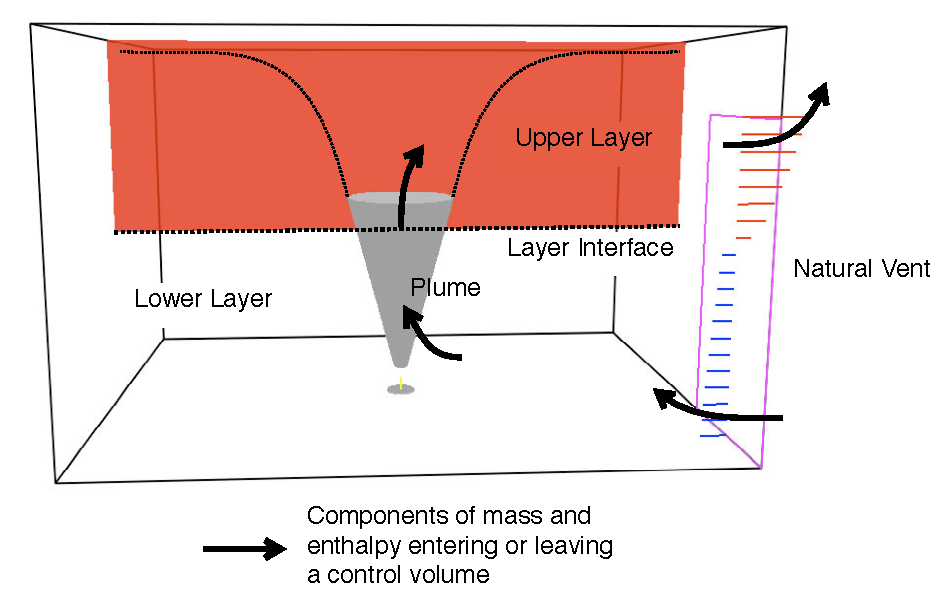
\includegraphics[width=\textwidth]{FIGURES/Theory/Control_Volumes}\\
\end{center}
\caption{Schematic of control volumes in a two-layer zone model.}
 \label{fig:Control_Volumes}
\end{figure}
Conservation of mass in each layer, $\dot m_i$, is expressed
\be
   \dbydt{m_i} = \dot m_i  \label{mass_con}
\ee
Conservation of energy takes the form of the first law of thermodynamics, which states that the rate of increase of internal energy plus the rate at which the layer does work by expansion is equal to the rate at which enthalpy is added to the gas:
\be
   \dbydt{(c_v m_i T_i)} +  P \dbydt{V_i} =  \dot h_i \label{eq:first_law}
\ee
The enthalpy source term, $\dot h_i$, consists of the fire's heat release rate, conduction losses to walls, and radiation exchange. The layer temperature and mass are related to the layer volume and compartment pressure via the ideal gas law:
\be
  P \, V_i = m_i \, R \, T_i \label{EoS}
\ee
A system of ordinary differential equations for the compartment pressure, upper layer volume, and layer temperatures can be derived from these three basic principles:
\begin{eqnarray}
\dbydt{P} &=& \frac{{\gamma-1}}{{V}} \left( \dhl + \dhu \right)  \\[.1in]
\dbydt{\Vu} &=& \frac{1}{P \gamma} \left( (\gamma-1) \, \dhu - \Vu \dbydt{P} \right) \\[.1in]
\dbydt{\Tu} &=& \frac{1}{c_p \, m_{\rm u}} \left( \dhu - c_p \, \dmau \, \Tu + \Vu \dbydt{P} \right) \\[.1in]
\dbydt{\Tl} &=& \frac{1}{c_p \, m_{\rm l}} \left( \dhl - c_p \, \dmau \, \Tl + \Vl \dbydt{P} \right)
\end{eqnarray}
As discussed in Refs.~\cite{Forney:1994} and \cite{Rehm:1992}, these equations are stiff, meaning that the pressure adjusts to changing conditions more quickly than the other variables. Runge-Kutta methods or predictor-corrector methods such as Adams-Bashforth require prohibitively small time steps in order to track the short time scale phenomena (pressure in our case). Methods that calculate the Jacobian (or at least approximate it) have a much larger stability region for stiff problems and are thus more successful at their solution.





\chapter{The Fire Plume}
\label{sec:TheFire}

Fires in CFAST are specified by the user in terms of a time-dependent heat release rate (HRR), an effective fuel molecule, and the yields of the products of incomplete combustion like soot and CO. Fires can be specified in multiple compartments and are treated as totally separate entities, with no interaction of the plumes. These fires are generally referred to as ``objects'' and can be ignited at a prescribed time, temperature or heat flux.

CFAST does not include a pyrolysis model to {\em predict}, as opposed to specify, the growth and spread of the fire. Rather, pyrolysis rates for each fire are prescribed by the user. While this approach does not directly account for increased pyrolysis due to radiative feedback from the flame or compartment, in theory these effects could be prescribed by the user. In an actual fire, this is an important consideration, and the specification used should consider the experimental conditions as closely as possible.

\section{Combustion Chemistry}

 The HRR of the fire is specified by the user, but it may be constrained by the availability of oxygen in the compartment. The combustion of a hydrocarbon fuel is described by the following single-step reaction:
\begin{eqnarray}
   \mathrm{C_{n_\C}H_{n_H}O_{n_O}N_{n_N}Cl_{n_{Cl}}} &+&  \nu_\OTWO \, \mathrm{O_2}  \rightarrow  \nonumber \\[.1in]
   \nu_\COTWO \, \mathrm{CO_2} &+& \nu_\HTWOO \, \mathrm{H_2O} \; + \; \nu_\CO \, \mathrm{CO} \; + \; \nu_\So \, \mathrm{Soot} \; + \; \nu_\HCl \mathrm{HCl} \; + \; \nu_\HCN \mathrm{HCN} \label{stoich}
\end{eqnarray}
The user specifies the composition of the fuel molecule and the yields of soot and CO, $y_\So$ and $y_\CO$, which are related to their stoichiometric coefficients as follows:
\begin{eqnarray}
   \nu_\So &=& \frac{M_\F}{M_\So} \; y_\So \label{soot_yield} \\[.1in]
   \nu_\CO &=& \frac{M_\F}{M_\CO} \; y_\CO \label{CO_yield}
\end{eqnarray}
Under the assumption that all of the nitrogen and chlorine in the fuel are converted to HCN and HCl, the other stoichiometric coefficients are:
\begin{eqnarray}
  \nu_\COTWO &=& \mathrm{n_\C} - \brackets{\nu_\CO + \nu_\HCN + \nu_\So} \\[.1in]
  \nu_\HTWOO &=& \frac{\mathrm{n_\Hy} - \brackets{\nu_\HCl + \nu_\HCN}}{2} \\[.1in]
  \nu_\OTWO  &=& \nu_\COTWO + \frac{\nu_\HTWOO + \nu_\CO - \mathrm{n_\Oh}}{2} \label{Oxygen_yield} \\[.1in]
  \nu_\HCl   &=& \mathrm{n_{Cl}} \\[.1in]
  \nu_\HCN   &=& \mathrm{n_{N}}
\end{eqnarray}
Note that the nitrogen in the air acts only as a diluent. The yields of hydrogen cyanide and hydrogen chloride are based solely on the composition of the fuel molecule. Finally, a user-specified trace species can be specified to follow the transport that results from fire-induced flow for an arbitrary species. This may be of particular interest for radiological releases \cite{Jones:2008}, but may be useful for any trace amounts released by a fire.

\section{Heat Release Rate}
\label{section:HRR}

As fuel and oxygen are consumed, heat is released and various products of combustion are formed. The heat is released as radiation and convected enthalpy:
\begin{eqnarray}
   \dQr &=& \chi_{\rm r} \, \dQ \\[.1in]
   \dQc &=& (1-\chi_{\rm r}) \, \dQ
\end{eqnarray}
where, $\chi_{\rm r}$ is the fraction  of the fire's heat release rate given off as radiation. The default value to 0.30~\cite{Drysdale:1985}.

While it is convenient for the user to directly specify the heat release rate of the fire, it is actually the pyrolysis rate of fuel, $\dmf$, that is specified:
\be
   \dmf = \frac{\dQ}{\Dh}
\ee
where $\Dh$ is the heat of combustion. In the event that the HRR is constrained by the availability of oxygen, the pyrolysis rate does not change, but the HRR becomes:
\be
   \dQ = \min \Big( \dmf \, \Dh \, , \, \dme \, Y_\OTWO \, C_{\rm LOL} \, \DhO \Big)
\ee
where $\dme$ is the entrainment rate, $Y_\OTWO$ is the mass fraction of oxygen in the layer containing the fire, $\DhO$ is the heat of combustion based on oxygen consumption\footnote{The heat of combustion based on oxygen consumption is taken to be 13.1~MJ/kg, representative of typical hydrocarbon fuels~\cite{Huggett:1980}.}, and $C_{\rm LOL}$ is the smoothing function ranging from 0 to 1:
\be
   C_{\rm LOL} = \frac{\tanh \Big( 800 (Y_\OTWO - Y_{\OTWO,{\rm l}}) - 4 \Big) + 1}{2}
\ee
The limiting oxygen mass fraction, $Y_{\OTWO,{\rm l}}$, is 0.1, by default.



\section{Plume Entrainment}

The plume mass entrainment, $\dme(z)$, at a height $z$ above the base of the fire is estimated using Heskestad's correlation~\cite{Heskestad:2002}:
\be
   \dme(z) = 0.196 \, \left( \frac{g \, \rho_\infty^2}{c_p \, T_\infty} \right)^{1/3} \, \dQ_{\rm c}^{1/3} \; \brackets{z - z_0}^{5/3} \;
   \left( 1 + \frac{2.9 \, \dQ_{\rm c}^{2/3}}{ \left( \sqrt{g} \, c_p \, \rho_\infty \, T_\infty \right)^{2/3} \, (z-z_0)^{5/3}} \right) \label{mdot_e}
\ee
where $z_0$ is a virtual origin defined as
\be
   \frac{z_0}{D} = -1.02 + 1.4 \, \dQ^{* \, 2/5} \quad ; \quad \dQ^* = \frac{\dQ}{\rho_\infty \, c_p \, T_\infty \, \sqrt{g \, D} \, D^2} \label{virtual_origin}
\ee
Note that the virtual origin is defined in terms of the total heat release rate of the fire, $\dQ$. Equation~(\ref{mdot_e}) is recommended above the mean flame height, $L$. Below the flame height, Heskestad recommends the following:
\be
  \dme(z) = \dme(L) \, \frac{z}{L} \quad ; \quad \frac{L}{D} = -1.02 + 3.7 \, \dQ^{* \, 2/5}
\ee
The mean flame height is defined as the distance from the fuel source to the top of the visible flame where the intermittency is 0.5.  A flame intermittency of 0.5 means that the visible flame is above the mean 50~\% of the time and below the mean 50~\% of the time.

In CFAST, there is a constraint on the mass entrainment rate because the plume can rise only so high for a given HRR.  Early in a fire, the plume may not have sufficient energy to reach the compartment ceiling. Therefore, a limit is placed on the entrainment rate. For the plume to be able to penetrate the hot upper layer, the density of the gas in the plume must be less than the density of the gas in the upper layer. This implies that the upper layer temperature must be less than the plume temperature:
\be
   \Tu < \Tp \approx \frac{ \dQc + \dme \, c_p \, \Tl }{ \dme \, c_p}
\ee
Rearranging terms yields a limit on the mass entrainment:
\be
   \dm_e < \frac{\dQc}{c_p (\Tu - \Tl)}
\ee


\section{Plume Centerline Temperature}

The centerline plume temperature rise, $\Delta T_0(z)$, at a height $z$ above the base of the fire is estimated using Heskestad's correlation~\cite{Heskestad:2002}:
\be
   \Delta T_0(z) = 9.1 \, \left( \frac{T_\infty}{g \, c_p^2 \, \rho_\infty^2} \right)^{1/3} \, \dQ_{\rm c}^{2/3} \, (z-z_0)^{-5/3}  \label{plume_temperature}
\ee
where the virtual origin, $z_0$, is defined in Eq.~(\ref{virtual_origin}). Equation~(\ref{plume_temperature}) is valid above the flame height, $L$, and below the hot gas layer interface, $z_{\rm I}$. Below the flame height, the temperature rise is approximated at 900~K. Above the layer interface, the temperature and density of the entrained air is significantly different than that of the lower layer. To account for this, the temperature correlation is modified for values of $z$ greater than the interface height, $z_{\rm I}$:
\be
   \Delta T_0(z) = 9.1 \, \left( \frac{\Tu}{g \, c_p^2 \, \rho_{\rm u}^2} \right)^{1/3} \, \dQ_{\rm c}^{2/3} \, (z-z_0')^{-5/3}  \quad ; \quad z>z_{\rm I}  \label{plume_temperature_upper}
\ee
where the modified virtual origin is given by:
\be
   z_0' = z_{\rm I} - \left( \frac{\Tu}{\Tl} \right)^{3/5} \, (z_{\rm I}-z_0)  \label{virtual_origin_modified}
\ee
Equations~(\ref{plume_temperature_upper}) and (\ref{virtual_origin_modified}) are obtained by asserting that $\Delta T_0$ is continuous across the layer interface and that $\Tu \rho_{\rm u} \approx \Tl \rho_{\rm l}$.

The mass entrainment correlation, Eq.~(\ref{mdot_e}), is modified the same way above the layer interface.



\chapter{Ventilation}

CFAST models three types of vent flow: natural flow through vertical vents (such as doors or windows),  natural flow through horizontal vents (such as ceiling holes or hatches), and forced flow via mechanical ventilation. Forced flow can occur through either vertical or horizontal vents.

Atmospheric pressure is about 100~kPa. Fires produce pressure changes from 1~Pa to 1~kPa and mechanical ventilation systems typically involve pressure differentials of about 1~Pa to 100~Pa.  The pressure variables are solved to a higher accuracy than other solution variables because of the subtraction (with resulting loss of precision) needed to calculate vent flows from pressure differences.


\section{Vertically-Oriented Vents (Doors and Windows)}

Natural flow through windows and doors is governed by the pressure difference across the opening.  A momentum equation for the zone boundaries is not solved directly.  Instead momentum transfer at the zone boundaries is included by using Bernoulli's equation augmented for restricted openings with an orifice coefficient~\cite{Quintiere:1984, Steckler_Coefficients}.

The mass flow through a vertical opening is calculated by dividing the vertical extent of the opening into discrete segments, each of which is bounded by either the top or bottom of the door or window, the zone interface of either compartment, or the neutral plane, which is where the velocity changes direction. In this way, the vent opening is partitioned into at most six sections.

Let $z=b$ and $z=t$ denote the height of the bottom and top of the segment, and $\Delta P_b$ and $\Delta P_t$ denote the pressure differences at those heights.  Because the segment is either completely above or completely below the neutral plane, the two pressure differences will have the same sign. The mass flow through the segment can then be computed by integrating from $b$ to $t$:
\begin{eqnarray}
\dm &=& \int_b^t C \sqrt{2 \rho \, \Delta P(z)} \, w \, dz  \\[.1in]
    &=& C\sqrt{2\rho} \, w \int_b^t\sqrt{\frac{|(t-z) \, \Delta P_b + (z-b) \, \Delta P_t|}{t-b}} \; dz \\[.1in]
    &=& \frac{2}{3} \, C \sqrt{2\rho} \, w \, (t-b)\frac{|\Delta P_t|^{3/2}-|\Delta P_b|^{3/2}}{|\Delta P_t|-|\Delta P_b|}
\label{eq:massflowone}
\end{eqnarray}
Here, $C$ is the orifice coefficient taken to be 0.7~\cite{Steckler_Coefficients}, $\rho$ is the gas density of the upwind compartment, and $\Delta P(z)$ is the pressure across the interface at elevation $z$. Note that the integral is evaluated from
\begin{eqnarray}
\int \sqrt{A+Bz} \, dz = \frac{2}{3B}(A+Bz)^{3/2}+\mbox{constant}
\end{eqnarray}
where $A=(|t\,\Delta P_t|-b\,|\Delta P_b|)/(t-b)$ and $B=(|\Delta P_t|-|\Delta P_b|)/(t-b)$.
Equation \ref{eq:massflowone} is sometimes written:
\be
   \dm = \frac{2}{3} C \sqrt{2 \rho} \, w \, (t-b)  \frac{|\Delta P_t|+\sqrt{|\Delta P_t \,\Delta P_b|}+|\Delta P_b|}{\sqrt{|\Delta P_t|}+\sqrt{|\Delta P_b|} }
\ee
The mass flows through the various vertical segments of the door or window are distributed into the upper and lower layers of the downstream compartment depending on the temperature of the stream. Consider the flow of gas from the upper layer of Compartment~1 entering the lower layer of Compartment~2 (see Fig.~\ref{fig:Flow_Patterns}).
\begin{figure}[t]
\setlength{\unitlength}{1in}
\begin{picture}(6.5,4)
\thicklines
\put(0,0){\line(1,0){6.5}}
\put(0,4){\line(1,0){6.5}}
\put(3.25,4){\line(0,-1){1}}
\thinlines
\put(0,1.5){\line(1,0){3.25}}
\put(3.25,2.5){\line(1,0){3.25}}
\put(0,2.0){\line(1,0){6.5}}
\put(3.5,0.75){\vector(-1,0){0.5}}
\put(3.5,1.75){\vector(-1,0){0.5}}
\put(3,2.25){\vector(1,0){0.5}}
\put(3,2.75){\vector(1,0){0.5}}

\put(1.625,3.8){\makebox(0,0){Compartment 1}}
\put(4.875,3.8){\makebox(0,0){Compartment 2}}
\put(6,1.85){\makebox(0,0){Neutral Plane}}
\put(5.95,2.35){\makebox(0,0){Layer Interface}}
\put(0,1.35){Layer Interface}
\put(3.75,0.75){\makebox(0,0){$\dm_{\rm l \to l}$}}
\put(3.75,1.75){\makebox(0,0){$\dm_{\rm l \to u}$}}
\put(2.75,2.25){\makebox(0,0){$\dm_{\rm u \to l}$}}
\put(2.75,2.75){\makebox(0,0){$\dm_{\rm u \to u}$}}

\end{picture}
\caption{Flow patterns for horizontal flow through a vertical vent.}
\label{fig:Flow_Patterns}
\end{figure}
The mass flow rate is denoted $\dm_{\rm u \to l}$, where the subscripts indicate the upstream and downstream layer indices, respectively. The enthalpy flow rate is:
\be
   \doh_{\rm u \to l} = c_p \brackets{T_{\rm u,1}-T_{\rm l,2}} \, \dm_{\rm u \to l}
\ee
Assuming that $T_{\rm l,2} < T_{\rm u,1} < T_{\rm u,2}$, this energy will be distributed between the compartment's two layers. The distribution is based on the relative difference in temperature between the incoming gas stream and the layer temperatures. Some of the energy stays within the lower layer and some of the energy goes to the upper layer in the form of a virtual plume. The effective heat release rate of this virtual plume is:
\be
   \dQ_{\rm eff} = \frac{T_{\rm u,1}-T_{\rm l,2}}{T_{\rm u,2}-T_{\rm l,2}} \; \doh_{\rm u \to l}
\ee
The mass entrainment rate into this virtual plume at the midpoint of the vertical segment, $\bar{z}$, is assumed to be a fraction of the incoming mass flow rate:
\be
   \dm_{\rm e,eff} = \frac{T_{\rm u,1}-T_{\rm l,2}}{T_{\rm u,2}-T_{\rm l,2}} \; \dm_{\rm u \to l}
\ee
The origin of the virtual plume, $z_0$, is deduced from the plume mass entrainment correlation, Eq.~\ref{mdot_e}. That is, $z_0$ is the origin of the virtual plume whose convective heat release rate is $\dQ_{\rm eff}$ and whose mass entrainment rate is $\dm_{\rm e,eff}$ at the midpoint of the segment, $\bar{z}$:
\be
   z_0 = \bar{z} - \dm_{\rm e,eff}^{3/5} \, \left[ 0.196 \, \left( \frac{g \, \rho_\infty^2}{c_p \, T_\infty} \right)^{1/3} \, \dQ_{\rm eff}^{1/3} \right]^{-3/5}
\ee

The other type of mixing is much like an inverse plume and causes contamination of the lower layer.  It occurs when there is flow of the type $\dm_{42} > 0$.  The shear flow causes vortex shedding into the lower layer and thus some of the particulates end up in the lower layer.  The actual amount of mass or energy transferred is usually not large, but its effect can be large.  For example, even minute amounts of carbon can change the radiative properties of the gas layer, from negligible to something finite.  It changes the rate of radiation absorption significantly and invalidates the simplification of an ambient temperature lower layer.  This term is predicated on the Kelvin-Helmholz flow instability and requires shear flow between two separate fluids.  The mixing is enhanced for greater density differences between the two layers. However, the amount of mixing has never been well characterized. Quintiere et al. \cite{Quintiere:1984} discuss this phenomena for the case of crib fires in a single room, but their correlation does not yield good agreement with experimental data in the general case \cite{Quintiere:1981}.  In the CFAST model, it is assumed that the incoming cold plume behaves like the inverse of the usual door jet between adjacent hot layers; thus we have a descending plume.  The same equations are used to calculate this inverse plume as are used for the upright door mixing, above. It is possible that the entrainment is overestimated in this case, since buoyancy, which is the driving force, is not nearly as strong as for the usually upright plume.

\section{Horizontally-Oriented Vents (Floor and Ceiling Vents)}

Flow through a ceiling or floor vent is governed by both pressure and density differences. The simplest form is uni-directional flow driven primarily by a relatively large pressure difference. When the pressure difference is relatively small, the density difference, where hot gas underlies colder gas, can lead to bi-directional flow where the gas in the lower compartment rises into the upper compartment and {\em vice versa}.  This situation might arise in a real fire if the room of origin suddenly has a hole open up in the ceiling.

Cooper's algorithm~\cite{Cooper:1989, Cooper:1990, Cooper:1995} is used for computing mass flow through ceiling and floor vents:
\be
   \dm = 0.1 \brackets{\frac{g \, \Delta \rho \, A_{\rm v}^{5/2}}{\rho_{\rm avg}}} \brackets{1 - \frac{2 \, A_{\rm v}^2 \, \Delta P}{S^2 \, g \, \Delta \rho \, D^5}}
\ee
where $D = 2 \sqrt{A_{\rm v} / \pi}$ and $S$ is 0.754 for round or 0.942 for square openings, respectively. For each layer on either side of the vent, there are two values of the mass flow, $\dm_{\rm in}$ and $\dm_{\rm out}$. These terms are symmetric: the outgoing flow from one compartment is the incoming flow to the other. The corresponding enthalpy flows are determined from the relative size and temperature of the lower and upper layers:
\begin{eqnarray}
  \doh_{\rm in} &=& c_p \, \dmu \, \Tu + c_p \, \dml \, \Tl \\[0.1in]
  \dmu &=& \dm_{\rm in} \, \frac{\Vu}{V} \\[0.1in]
  \dml &=& \dm_{\rm in} \, \frac{\Vl}{V}
\end{eqnarray}
The mass and energy are then deposited into the upper or lower layer of the receiving compartment based on the effective temperature of the incoming flow relative to the upper and lower layers of the receiving compartment. If the temperature of the incoming flow is higher than the temperature of the lower layer, then the flow is deposited into the upper layer. This is similar to the idea of using a virtual plume for a doorway flow.


\section{Forced Flow}

CFAST models mechanical ventilation in terms of user-specified volume flows at various points in the compartment. The model does not include duct work or fan curves. These equations are high-order, non-linear and in some cases ill-posed, which caused a great deal of difficulty in reaching a numerical solution.

Figure~\ref{fig:Fans_and_Ducts}(a) depicts smoke exhaust via a fan at the top of an atrium, and Fig.~\ref{fig:Fans_and_Ducts}(b) illustrates a kitchen exhaust fan.  Cross ventilation, shown in Fig.~\ref{fig:Fans_and_Ducts}(c), is occasionally used without heating or cooling.  Generally systems that maintain comfort conditions have either one or two fans. Further information about these systems is presented in Klote and Milke~\cite{Klote:2002} and the American Society of Heating, Refrigerating and Air Conditioning Engineers (ASHRAE) \cite{ASHRAE:2001}.

\begin{figure}
\begin{center}
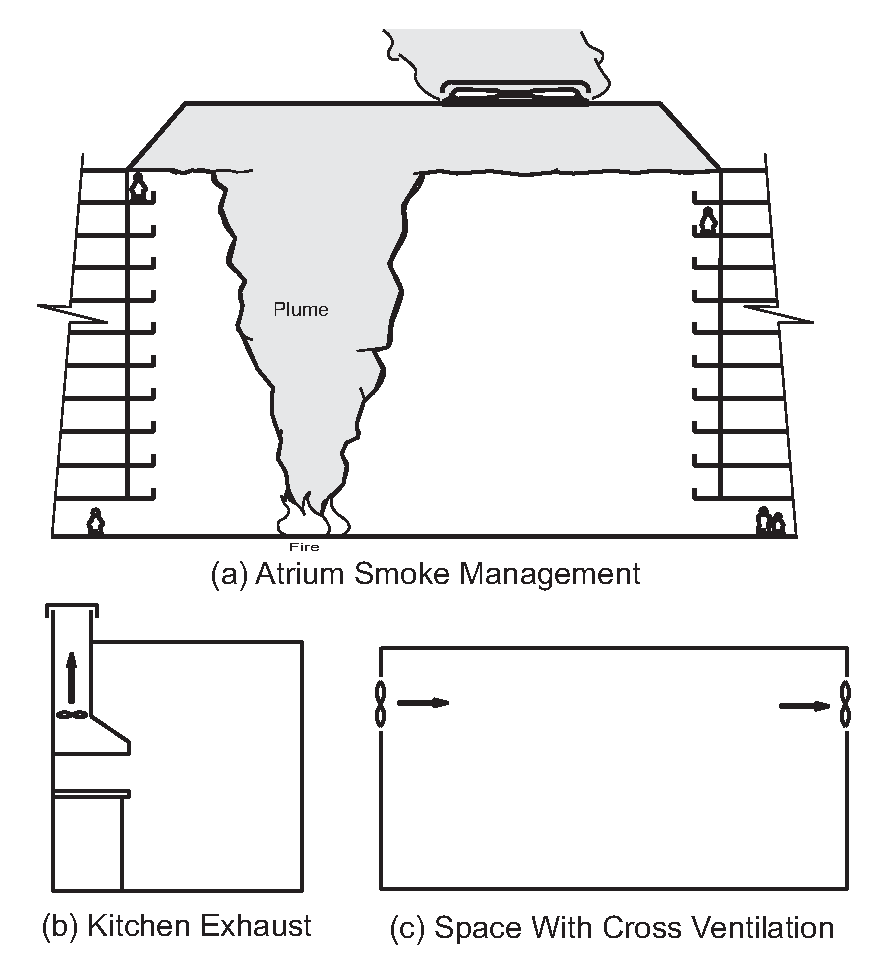
\includegraphics[width=5.0in]{FIGURES/Theory/HVAC_Fans_and_Ducts}\\
\end{center}
\caption{Some simple fan-duct systems.}
 \label{fig:Fans_and_Ducts}
\end{figure}

The flow through mechanical vents can be filtered. Filtering affects particulates such as smoke and the trace species. Filtering can be turned on at any time. Effectiveness is from 0~\% (no effect) to 100~\% which completely blocks flow of these two species.





\chapter{Heat Transfer}

This section discusses thermal radiation, convection and conduction, the three mechanisms by which heat is transferred between the gas layers and the enclosing compartment walls. Hot gases exchange heat with solid surfaces via convection and radiation. Heat is transferred through solids via conduction. Different material properties can be used for the ceiling, floor, and walls of each compartment (although all the walls of a compartment must be the same).  Additionally, each surface can be composed of up to three distinct layers.  This allows the user to deal naturally with the actual building construction.  Material thermophysical properties are assumed to be constant. Radiative transfer occurs among the fire(s), gas layers and compartment surfaces (ceiling, walls and floor).  This transfer is a function of the temperature differences and the emissivity of the gas layers as well as the compartment surfaces.  Typical surface emissivity values only vary over a small range.  For the gas layers, however, the emissivity is a function of the concentration of species which are strong radiators, predominately smoke particulates, carbon dioxide, and water.

\section{Radiation}
\label{sec:Radiation}

Radiation heat transfer is calculated between the ceiling, floor, wall layers, and fire, with the inclusion of emission and absorption by the hot gas layer~\cite{Forney_radiation}. The following assumptions are made:
\begin{itemize}
\item Each gas layer and each wall segment is assumed to be at a uniform temperature.
\item The wall and gas layer temperatures are assumed to change slowly over the duration of the time step of the governing equations.
\item The fire is assumed to radiate uniformly in all directions emitting a fraction, $\chi_{\rm r}$, of the total heat release rate.  This radiation is assumed to originate from a single point.  Radiation feedback to the fire and radiation from the plume is not modeled in the radiation exchange algorithm.
\item The radiation emitted is assumed to be diffuse and gray.  In other words, the radiant fluxes emitted are independent of direction and wavelength. At a solid surface, the emittance, $\epsilon$, absorptance, $\alpha$ and reflectance, $\rho$, are related via $\epsilon = \alpha = 1 - \rho$. In the gas phase, the emittance, $\epsilon$, absorptance, $\alpha$ and transmittance, $\tau$, are related via $\epsilon = \alpha = 1 - \tau$.
\item Rooms or compartments are assumed to be rectangular boxes.  Each wall is either perpendicular or parallel to every other wall.  Radiation transfer through vent openings is lost from the room.
\end{itemize}
The compartment lining is divided into four parts: the ceiling, the floor, and the wall sections above and below the layer interface. The net radiative heat flux at surface~$k$, $\dq_k''$, is found by solving the simplified radiation transport equation given by Eq.~(17-20) in Siegel and Howell~\cite{SiegelandHowell:1981}:
\be
   \frac{\dq_k''}{\epsilon_k} - \displaystyle\sum_{j=1}^N \frac{1 - \epsilon_j}{\epsilon_j} \, \dq_j'' \, F_{k-j} \, \tau_{k-j} = \sigma T_k^4 - \displaystyle\sum_{j=1}^N \brackets{\sigma T_j^4 \, F_{k-j} \, \tau_{k-j}} - c_k \label{RTE}
\ee
where $F_{k-j}$ is the configuration factor (fraction of radiant energy emitted by surface $j$ that is intercepted by surface $k$), $\tau_{k-j}$ is the transmittance, $\sigma$ is the Stefan-Boltzman constant, $\epsilon_k$ is the emissivity, $A_k$ is the area, and $T_k$ is the temperature of surface $k$. The radiation from the hot gas layer and the fire is included in the last term:
\be
   c_k = \epsilon_{\rm u} \, F_{{\rm u}-k} \, \sigma \, \Tu^4 + \frac{\omega_{{\rm f}-k}}{4 \pi} \frac{\chi_{\rm r} \, \dQ}{A_k}  \label{ckeq}
\ee
where $\epsilon_{\rm u}$ is the emittance (absorptance) of the upper layer, $F_{{\rm u}-k}$ is the view factor between the upper layer and solid surface, $\omega_{{\rm f}-k}$ is the solid angle between the fire and wall\footnote{Note that as the area of surface $k$ shrinks to zero, $\omega_{{\rm f}-k}/A_k \to 1/R^2$, yielding the classic point source radiation model}, and $\dQ$ is the heat release rate of the fire. If the solid surface, $k$, is the floor or the lower wall, the view factor refers to the layer interface. If the solid surface, is the upper wall or ceiling, the view factor is 1.

Reference~\cite{Forney_radiation} describes the solution of Eq.~\ref{RTE}.


\subsubsection{Configuration Factors}

The configuration factor, $F_{1-2}$, is the fraction of radiant energy emitted by surface 1 that is intercepted by  surface 2, and is calculated:
\be
   F_{1-2} = \frac{1}{A_1} \int_{A_1} \int_{A_2} \frac{\cos \theta_1 \, \cos \theta_2}{\pi L^2} \, dA_2 \, dA_1 \label{eq:config_factor}
\ee
where $L$ is the distance along the line of integration,  $\theta_1$ and $\theta_2$ are the angles for surface 1 and 2 between the respective normal vectors and the line of integration, and $A_1$ and $A_2$ are the areas of the two surfaces.  These terms are illustrated in Fig.~\ref{fig:Rad_Config_Factor}.  
\begin{figure}
\begin{center}
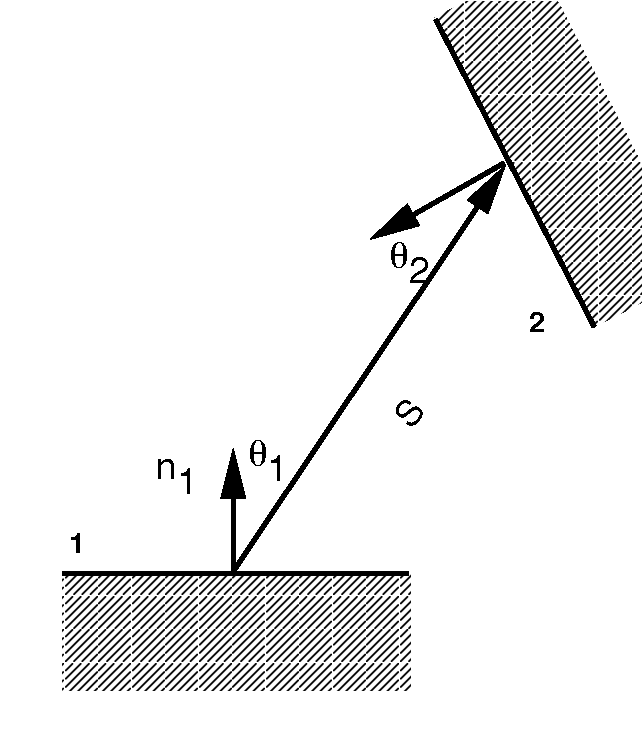
\includegraphics[width=3.0in]{FIGURES/Theory/Radiation_Config_Factor}\\
\end{center}
\caption{Setup for a configuration factor calculation between two arbitrarily oriented finite areas.}
 \label{fig:Rad_Config_Factor}
\end{figure}
There are two types of configuration factors in CFAST. First, consider two rectangles perpendicular to each other having a common edge of the same length, $l$. The dimension of the source rectangle is $l \times w$ and the target rectangle is $l \times h$. The configuration factor from source to target is:
\begin{eqnarray}
\lefteqn{F_{1-2} = \frac{1}{\pi \, W} \left[ W \, \tan^{-1} \frac{1}{W} + H \, \tan^{-1} \frac{1}{H} - \sqrt{H^2+W^2} \, \tan^{-1} \frac{1}{\sqrt{H^2+W^2}} + \right.}  \nonumber \\[.1in]
& &   \left. \frac{1}{4} \, \ln \left\{ \frac{(1+W^2)(1+H^2)}{1+W^2+H^2} \, \left( \frac{W^2(1+W^2+H^2)}{(1+W^2)(W^2+H^2)} \right)^{W^2} \left( \frac{H^2(1+W^2+H^2)}{(1+H^2)(W^2+H^2)} \right)^{H^2} \right\} \right]
\end{eqnarray}
where $H=h/l$ and $W=w/l$. 

Next, consider two identical, parallel, directly opposed rectangles. The dimension of the rectangles is $a \times b$ and the separation distance is $c$. The configuration factor is:
\begin{eqnarray}
\lefteqn{F_{1-2} = \frac{2}{\pi \, X \, Y} \left\{ \ln \left[ \frac{(1+X^2)(1+Y^2)}{1+X^2+Y^2} \right]^{1/2} + X \sqrt{1+Y^2} \, \tan^{-1} \frac{X}{\sqrt{1+Y^2}} + \right.} \nonumber \\[.1in]
& & \left. Y \sqrt{1+X^2} \, \tan^{-1} \frac{Y}{\sqrt{1+X^2}} - X \, \tan^{-1} X - Y\, \tan^{-1} Y \right\}
\end{eqnarray}
where $X=a/c$ and $Y=b/c$. These formulae are found in Appendix~C of Ref.~\cite{SiegelandHowell:1981}.

Next, the normalized solid angle, $\omega_{\rm f-k}$, in Eq.~(\ref{ckeq}) is computed. First, place a sphere of radius, $r$ tangent to a rectangle of dimension $x \times y$ such that the point of tangency is the corner of the rectangle. The normalized solid angle formed by the center of the sphere and the edges of the rectangle is given by: 
\be
   \omega(x,y;r) = \frac{1}{4\pi} \left[ \sin^{-1} \left( \frac{A \, y}{\sqrt{y^2+r^2}} \right) + \sin^{-1} \left( \frac{A \, x}{\sqrt{x^2+r^2}} \right) - \frac{\pi}{2} \right] \quad ; \quad A=\sqrt{1+\frac{r^2}{x^2+y^2}}
\ee
Suppose now that the radiation of a fire is assumed to emanate from a point a distance $r$ above the floor whose dimension is $L \times W$. Suppose also that the floor is divided into four quadrants based on the location of the fire. The dimensions are partitioned $L=L_1+L_2$ and $W=W_1+W_2$. The normalized solid angle between the point source fire, f, and the floor, fl, is: 
\be
   \omega_{\rm f-fl} = \sum_{j=1}^2 \sum_{i=1}^2 \omega(L_i,W_j;r)
\ee

\subsubsection{Transmittance and Absorptance}

The transmittance is the fraction of radiant energy that will pass through a volume filled with an absorbing media. It is usually expressed in the form:
\be
   \tau = {\rm e}^{-a L}
\ee
where $a$ is the absorption coefficient and $L$ is the path length. The absorptance is the fraction of radiant energy absorbed by that volume. For a gray gas, $\alpha + \tau = 1$.

In general, the transmittance and absorptance are functions of wavelength. This is an important factor to consider for the major gaseous products, $\textnormal{CO}_2$  and $\textnormal{H}_2 \textnormal{O}$. However soot has a continuous absorption spectrum that allows the transmittance and absorptance to be approximated as ``gray'' \cite{SiegelandHowell:1981} across the entire spectrum. The total transmittance over a path length $L$ through a volume of combustion products is taken as the product of the transmittance of the soot and major product gases:
\be
   \tau = e^{-a_{\rm s}L} \brackets{1 - \alpha_{\rm H_2O} - 0.5 \, \alpha_{\rm CO_2}}
\ee
The factor of 0.5 applied to the absorptance of CO$_2$ accounts for the overlap of the wavelength bands of the two gases. Tien~et~al.~\cite{Tien:2002} suggest that the absorption coefficient for soot may be approximated $a_{\rm s} = k f_v T$ where $k$ is a constant that depends on the optical properties of the soot particles, $f_v$ is the soot volume fraction, and $T$ is the (absolute) temperature. Values of $k$, have been found to be about constant for a wide range of fuels~\cite{Tien:1978}.

Absorptance data for $\textnormal{H}_2 \textnormal{O}$ and $\textnormal{CO}_2$ are reported in Ref.~\cite{Edwards:1985}. For each gas, these data are tabulated in a look-up table, implemented as a two-dimensional array based on temperature and gas concentration.

The effective path length, $L$, for the upper gas layer is approximated to be 1.8 times its depth~\cite{Tien:2002}.




\section{Convection}

The transfer of heat between the gas and solid surfaces is handled slightly differently at the ceiling, floor and walls, due to the difference in orientation and the presence of a relatively thin hot flow near the ceiling known as the ceiling jet. The following two sections describe how the convective heat transfer is done for these different surfaces.

\subsection{Walls and Floor}

In general, the convective heat flux to a solid surface is given by:
\be
   \dqc'' = h \, \brackets{\Tg - \Ts}  \label{convective_heat_flux}
\ee
The convective heat transfer coefficient, $h$, is a function of the gas properties, temperature, and velocity. In CFAST, simple correlations for natural convection are used since the gas velocity is unknown:
\be
   h = C {|\Tg - \Ts|}^{1/3}
\ee
where $C$ is an empirical coefficient (1.52 for the floor and ceiling (in the absence of a ceiling jet) and 1.31 for the walls~\cite{Holman:1990}), $\Tg$ is the average gas layer temperature adjacent to the surface, and $\Ts$ is the surface temperature.

\subsection{Ceiling}

During the early stage of a fire before a hot gas layer has formed, the convective heat transfer to the ceiling is governed by the temperature and velocity of the ceiling jet. Alpert's chapter in the {\em SFPE Handbook}~\cite{Alpert:SFPE} presents an empirical correlation for the convective heat flux from the ceiling jet to a relatively cool surface:
\be
   \dqc'' = 1.323 \, f \, \frac{\dQ_{\rm c}}{H^2} \, \left( \frac{r}{H} \right)^{-1.36}  \label{eq:cjflux}
\ee
where $f$ is a friction factor estimated to be 0.03, $r$ is the radial distance to the plume centerline, $H$ is the ceiling height, and $\dQ_{\rm c}$ is the convective fraction of the heat release rate. The average convective heat flux to the ceiling can be obtained by integrating this expression over the entire ceiling:
\be
   \dq_{\rm c,avg}'' = \frac{1}{LW} \int_0^{2\pi} \int_0^R \dqc'' \, r \, dr \, d\theta = \frac{0.27 \, \dQ_{\rm c}}{(LW)^{0.68} \, H^{0.64}} \label{eq:cjfluxavg}
\ee
Note that the integration is carried out over a circle whose area, $\pi R^2$, is equal to the area of the ceiling, $LW$.

Equation~(\ref{eq:cjfluxavg}) applies to the early stage of the fire; thus, a modified heat transfer coefficient is used so that there is a transition from the early to later stages when a layer has formed:
\be
   h = \max \left( \frac{\dq_{\rm c,avg}''}{\Tu-\Ts} \, , \, C {|\Tu - \Ts|}^{1/3} \right)
\ee
Here, $\Tu$ is the average temperature of the upper layer and $\Ts$ is the ceiling surface temperature. Notice that the rightmost term is simply the correlation used for the walls and floor.

\section{Conduction}

The heat conduction equation is solved in the direction normal to solid target or wall surfaces using non-uniformly spaced nodes and a second order accurate central difference scheme for the spatial derivatives and a semi-implicit time marching scheme. At each time step, the internal solid temperatures are updated in time until the net convective and radiative heat flux striking the wall equals with the heat flux into the solid~\cite{Moss:1992}:
\be
   \dq'' \equiv \dqr'' + \dqc'' = -k \, \frac{dT}{dx} \Big|_{x=0}
\ee
where $k$ is the thermal conductivity of the solid.  This solution strategy requires a differential algebraic equation (DAE) solver that can simultaneously solve both differential and algebraic equations.  With this method, only one or two extra equations are required per wall segment (two if both the interior and exterior wall segment surface temperatures are computed).  This solution strategy is more efficient than the method of lines since fewer equations need to be solved. Conduction is then coupled to the gas phase energy exchange.

A non-uniform array of internal nodes is used to capture steep gradients in temperature near the surface. Define a penetration depth of
\be
   x_p = 2 \sqrt{\alpha \, t_{\rm end}} \; \hbox{erfc}^{-1} \brackets{0.05}
\ee
where $\hbox{erfc}^{-1}$ denotes the inverse of the complementary error function. The value $x_p$ is the location in a semi-infinite wall where the temperature rise is 5~\% after $t_{\rm end}$ seconds. Eighty percent of the nodes are placed on the interior side of $x_p$ and the remaining 20~\% are placed on the exterior side.

The heat conduction equation normal to the solid surface is:
\be \frac{\partial T}{\partial t} = \frac{k}{\rho c}\frac{\partial^2 T}{\partial x^2}
\label{eq:Target_PDE} \ee
where $k$, $\rho$ and $c$ are the thermal conductivity, density and heat capacity of the target. At the surface, $x=0$, the boundary condition is:
\be
   \dq''=-k\frac{dT}{dx} \label{eq:Target_Fourier}
\ee
where $\dq''$ is the net convective and radiative heat flux.

\newcommand{\Dt}{\Delta t}
\newcommand{\Dr}{\Delta r}
\newcommand{\Tipo}{T_{i+1}^{n+1}}
\newcommand{\Ti}{T_{i}^{n+1}}
\newcommand{\Timo}{T_{i-1}^{n+1}}

The 1-D heat conduction equation can be solved in either Cartesian or cylindrical coordinates. The solution methodology shall be presented for cylindrical coordinates:
\be 
  \frac{\partial T}{\partial t} = \frac{k}{\rho c} \frac{1}{r} \frac{\partial}{\partial r} \left( r \frac{\partial T}{\partial r} \right)
\ee
Dividing the cylinder into $N$ uniformly spaced concentric control volumes, this equation can be written in discretized form:
\begin{eqnarray}
\Ti-T_i^n&=& \frac{\Dt}{\Dr} \frac{k}{\rho c}
\left[
\left(\frac{\Tipo-\Ti}{\Dr}\right)
\frac{r_i}{r_{i-1/2}}-
\left(\frac{\Ti-\Timo}{\Dr}\right)
\frac{r_{i-1}}{r_{i-1/2}}
\right]
\nonumber\\[0.2in]
&=&\frac{\Dt \, \alpha}{\Dr^2}
\left[
\left(\Tipo-\Ti\right)
\left(\frac{i}{i-0.5}\right)-
\left(\Ti-\Timo\right)
\left(\frac{i-1}{i-0.5}\right)
\right]
\label{eq:cylheat6}
\end{eqnarray}
where $\alpha=k/(\rho c)$. Defining $C_i$ and $D_i$ as
\be
C_i = \frac{\alpha\Dt}{\Dr^2}\left(\frac{i-1}{i-0.5}\right) \quad ; \quad D_i = \frac{\alpha\Dt}{\Dr^2}\left(\frac{i}{i-0.5}\right)
\ee
Eq.~(\ref{eq:cylheat6}) can be written:
\be
-C_i \, \Timo + \left( 1+2\frac{\alpha\Dt}{\Dr^2} \right) \, \Ti - D_i \, \Tipo = T_i^n  \quad \quad i=1...N-1
\label{eq:cylheat8}
\ee
The boundary condition is applied at control volume $N$:
\begin{eqnarray*}
T_N^{n+1}-T_N^n=\frac{\alpha\Dt}{\Dr^2}
\left[\frac{\Dr \, \dq''}{k} \frac{N}{N-0.5} -(T_N^{n+1}-T_{N-1}^{n+1}) \frac{N-1}{N-0.5} \right]
\end{eqnarray*}
or
\be
-C_N \, T_{N-1}^{n+1}+ \left( 1+C_N \right) T_N^{n+1} = T_N^n+D_N\frac{\Dr}{k} \dq''
\label{eq:cylheat10}
\ee
The internal temperature profile, $T_i$, is then obtained with a tri-diagonal linear solver.




\section{Coupling the Gas and Solid Phase Calculations}

To illustrate the method, consider a one room case with one active wall.  There are four gas phase equations (pressure, upper layer volume, upper and lower layer temperatures) and one wall temperature equation.  Implementation of the gradient matching method requires that storage be allocated for the temperature profiles at the current time step, $t$, and at the next time step, $t + \Delta t$.  Given the profile at time $t$ and values for the five unknowns at time $t + \Delta t$ (initial guess by the solver), the temperature profile is advanced from time $t$ to $t + \Delta t$.  The temperature gradient at the wall surface is computed followed by the residuals for the five equations.  The DAE solver adjusts the solution variables and the time step until the residuals for all the equations are below an error tolerance.  Once the solver has completed the step, the array storing the temperature profile for the previous time is updated, and the DAE solver is ready to take its next step.

Heat transfer between connected compartments is modeled by merging the back surfaces of the connected ceiling and floor of the compartments or the back wall surfaces of the connected horizontal compartments.  A heat conduction problem is solved for the merged walls using a temperature boundary condition for both the near and far wall.  As before, temperatures are determined by the DAE solver so that the heat flux striking the wall surface (both interior and exterior) is consistent with the temperature gradient at that surface.

For horizontal heat transfer between compartments, the connections may be between partial wall surfaces, expressed as a fraction of the wall surface. CFAST first estimates conduction fractions analogous to radiation configuration factors. For example, if only one half of the rear wall in one compartment is adjacent to the front wall in a second compartment, the conduction fraction between the two compartments is 0.5. Once these fractions are determined, an average flux, $\dq_{\rm avg}''$, is calculated using
\be
   \dq_{\rm avg}'' = \sum_{\rm walls} \, F_{i-j} \, \dq_j''
\ee
where $F_{ij}$ is the fraction of flux from wall $i$ that contributes to wall $j$, $\dq_j''$ is the flux striking wall $j$.



\chapter{Fire Protection Devices}



\section{Sprinkler and Heat Detector Activation}

The link temperature of a sprinkler or heat detector is modeled using the differential equation~\cite{Heskestad:1976}:
\be
   \frac{d \TL}{dt} = \frac{\sqrt{v}}{\rm RTI} \brackets{\Tg - \TL}  \label{eq:RTI}
\ee
where $\TL$ and $\Tg$ are the link and gas temperatures, $v$ is the ceiling jet velocity, and RTI (Response Time Index) is a measure of the sensor's thermal inertia. The gas temperature and velocity obtained from the ceiling jet algorithm, described below. Rooms without fires do not have ceiling jets, in which case the upper layer temperature is used, along with a fixed velocity of 0.12~m/s. The link and gas temperatures and the velocity are functions of time; the RTI is a constant for a given detector type. The detector equation is solved numerically using the semi-implicit updating scheme:
\be
   \frac{\TL^{n+1}-\TL^n}{\delta t} = \frac{1}{2} \left( \frac{\sqrt{v^n}}{\rm RTI} \brackets{\Tg^n - \TL^n}  + \frac{\sqrt{v^{n+1}}}{\rm RTI} \brackets{\Tg^{n+1} - \TL^{n+1}}  \right) \label{eq:RTI_rewritten}
\ee
where the superscript $n$ denotes the value at the current time, and $\delta t$ is the time step.

The local gas velocity and temperature are estimated assuming the ceiling jet is immersed in a hot gas layer. From the work of Cooper \cite{Cooper:1990b}:
\be
   \frac{v_{cj}}{v_{max}} = \left\{ \begin{array}{r@{\quad \quad}l}
  \brackets{\zdel}^{1/7}\brackets{8-\zdel}/7 &  0 \leq \zdel<1 \\[.1in]
   \cosh{\brackets{c_r \brackets{\zdel-1}}}^2 &  1 \leq \zdel \end{array} \right.
\ee

\be
  \Theta = \frac{T_{CJ}-T_U}{T_{max}-T_U}= \left\{ \begin{array}{r@{\quad \quad}l}
   \Theta_s+ 2 \brackets{1-\Theta_s}\zdel - \brackets{1-\Theta_s}\brackets{\zdel}^2 &  0 \leq \zdel<1 \\[.1in]
   \frac{v_{cj}}{v_{max}} &  1 \leq \zdel \end{array} \right.
\ee
where $v_{max}=0.85\brackets{r/H}^{-1.1}\sqrt{gH}\sqrt[3]{Q_H^*}$, $Q_H^*= \dQ/\brackets{\rho_U c_p T_U \sqrt{gH} H^2}$, $\delta/H=0.1\brackets{r/H}^{0.9}$, $c_r=\frac{0.23}{0.77}\log{\brackets{\sqrt{2}-1}}$, $T_{max}=T_U + 2.6\brackets{1-\lambda_c}\brackets{r/H}^{-4/5}\brackets{Q_H^*}^{2/3}T_U - 0.09 \brackets{T_s-T_U}$, $\Theta_s=\Theta\brackets{T_{CJ}=T_s}$ and $\lambda_c$ is the fraction of the fire's heat release transferred by convection to the ceiling from the point of impingement to $r$, evaluated numerically. If the detector or sprinkler is outside the ceiling jet layer or in a compartment without a fire, the appropriate gas layer temperature and a default velocity of 0.1 m/s is used.

\section{Fire Suppression} \label{sec:suppression}

Fire suppression by water is predicted using a simple empirical model developed by Madrzykowski \cite{Madrzykowski:1992} and Evans~\cite{Evans:1993}. After activation of the sprinkler, $t > t_{\rm act}$, the heat release rate is assumed to decrease exponentially:
\be
   \dQ(t) = \dQ(t_{\rm act}) \; {\rm e}^{-(t-t_{\rm act}) /\tau}   \quad ; \quad \tau = 3 u_{\rm w}^{-1.8}
\ee
where $u_{\rm w}$ is the water spray density, expressed in units of m/s. The product species mass production rates are reduced by the same amount as the heat release rate.

There are assumptions and limitations in this approach. Its main deficiency is that it assumes that sufficient water is applied to the fire to cause a decrease in the rate of heat release. This suppression model cannot handle the case when the fire overwhelms the sprinkler.  The suppression model as implemented does not include the effect of a second sprinkler. Detection of all sprinklers are noted but their activation does not make the fire go out any faster. Further, multiple fires in a room imply multiple ceiling jets. It is not clear how the two ceiling jets should interact. When there is more than one fire, the detection algorithm uses the fire that results in the highest ceiling jet temperature in order to calculate the sprinkler link temperature.

\section{Species Concentration and Deposition}

CFAST uses a combustion chemistry scheme based on a carbon-hydrogen-oxygen balance.  The scheme is applied in three places.  The first is burning in the portion of the plume which is in the lower layer of the compartment of fire origin.  The second is the portion in the upper layer, also in the compartment of origin.  The third is in the vent flow which entrains air from a lower layer into an upper layer in an adjacent compartment.  Included in the combustion calculation is the generation and transport of a number of species that may be produced by a fire.  These species include unburned fuel, nitrogen, oxygen, carbon monoxide, carbon dioxide, hydrogen, carbon (assumed to be soot produced by the fire), hydrogen cyanide, hydrogen chloride, and an arbitrary trace species.

\subsection{Species Transport}

The species transport in CFAST is primarily a matter of bookkeeping to track individual gas species layer to layer and compartment to compartment. When the gas layers are initialized at the start of the simulation, they are set to ambient conditions.  These are the initial temperature prescribed by the user, and 23~\% by mass fraction (21~\% by volume fraction) oxygen, 77~\% by mass fraction (79~\% by volume fraction) nitrogen, a mass concentration of water prescribed by the user as a relative humidity, and a zero concentration of all other species.  As fuel is burned, the various species are produced in direct proportion to the mass of fuel burned (this relation is the species yields prescribed by the user for the fuel burning).  Since oxygen is consumed rather than produced by the burning, the `yield' of oxygen is negative, and is set internally to correspond to the amount of oxygen used to burn the fuel (within the constraint of available oxygen limits discussed in Section~\ref{section:HRR}). Two special separate species calculations are included in the model, a time-integrated value for a generic toxic species, Ct, and an arbitrary trace species, TS.  Both are assumed not to be part of the overall mass balance, but are rather generated by a fire and transported in a manner identical to other species.

Each unit mass of a species produced by a fire is carried in the flow to the various rooms and accumulates in the layers.  The model keeps track of the mass of each species in each layer, and knows the volume of each layer as a function of time.  The mass divided by the volume is the mass concentration, which along with the relative molecular mass gives the concentration in volume percent or parts per million as appropriate. Filters can be used in mechanical ventilation systems to remove species. The phenomenon has been implemented in CFAST to remove trace species and soot. It is implemented by modifying the source terms which describe gas flow. Mass that is filtered remains on the filter and is removed from the air stream. Both the resulting species density and total species removed can be analyzed. See Ref.~\cite{Jones:2008} for an example on the use of filtering.

The calculation of radiation exchange in CFAST also depends in part on the species concentrations calculated by the model (and thus the user inputs for species yields). There are two separate radiation calculations done by CFAST. The first is for broadband radiation transfer for energy balance. The way this calculation is done is discussed in Section~\ref{sec:Radiation}. The second is a visible light calculation to answer the question of whether exit signs will be visible. The absorption of broadband radiation depends on the concentration of water, carbon dioxide and soot. The visibility calculation depends solely on the soot concentration For soot, the input for soot yield  assumes all the excess carbon goes to soot). This soot generation is then transported as a species to yield a soot mass concentration to use in the optical density calculation based originally on the work of Seader and Einhorn~\cite{Seader:1976}. The most recent work is by Mulholland and Croakin~\cite{Mullholland:2000}. Based on their experimental measurements, the soot mass density is multiplied by 3,817~m\superscript{2}/kg (formerly 3,500~m\superscript{2}/kg) to obtain an optical density (in units of m\superscript{-1}) which is the value reported by the model.

\subsection{HCl Deposition}\label{HClDeposition}

Hydrogen chloride produced in a fire can produce a strong irritant reaction that can impair escape from the fire.  It has been shown \cite{Galloway:1989} that significant amounts of the substance may be removed by adsorption by surfaces which contact smoke.  In our model, HCl production is treated in a manner similar to other species.  However, an additional term is required to allow for deposition on, and subsequent absorption into, material surfaces.

The physical configuration that we are modeling is a gas layer adjacent to a surface (Fig.~\ref{fig:HCl_Deposition}).  The gas layer is at some temperature $T_g$ with a concomitant density of hydrogen chloride, $\rho_{HCl}$.  The mass transport coefficient is calculated based on the Reynolds analogy with mass and heat transfer; that is, hydrogen chloride is mass being moved convectively in the boundary layer, and some of it simply sticks to the wall surface rather than completing the journey during the convective roll-up associated with eddy diffusion in the boundary layer.  The boundary layer at the wall is then in equilibrium with the wall.  The latter is a statistical process and is determined by evaporation from the wall and stickiness of the wall for HCl molecules.  This latter is greatly influenced by the concentration of water in the gas, in the boundary layer and on the wall itself.

\begin{figure}[h]
\begin{center}
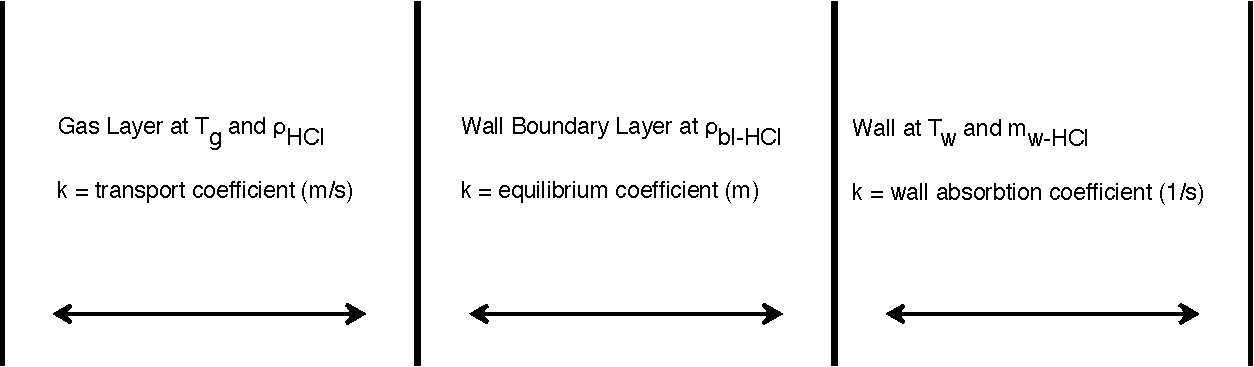
\includegraphics[width=5.0in]{FIGURES/Theory/HCl_Deposition}\\
\end{center}
\caption{Schematic of hydrogen chloride deposition region.}
 \label{fig:HCl_Deposition}
\end{figure}

The rate of addition of mass of hydrogen chloride to the gas layer is given by

\be \frac{d}{dt} m_{HCl} = source - k_c \brackets{\rho_{HCl} - \rho_{bl-HCl}} A_w \ee
where source is the production rate from the burning object plus flow from other compartments. For the wall concentration, the rate of addition is

\be \frac{d}{dt} d_{w-HCl} = k_c \brackets{\rho_{HCl} - \rho_{bl-HCl}} - k_s m_{w-HCl} \ee
where the concentration in the boundary layer, $\rho_{bl-HCl}$  is related to the wall surface concentration by the equilibrium constant $k_e$, by the relation $\rho_{bl-HCl} = d_{w-HCl} / k_e$. We never actually solve for the concentration in the boundary layer, but it is available, as is a boundary layer temperature if it were of interest.  The transfer coefficients are

\be k_c = \frac{\dot{q}}{\Delta T \rho_g c_p} \ee
\be k_e = \frac{b_1 e^{1500/T_w}}{1 + b_2 e^{1500/T_w} \rho_{HCl}} \brackets{1 + \frac{b_5 \brackets{\rho_{H_2O}}^{b_6}}{\brackets{\rho_{H_2O,sat} - \rho_{H_2O,g}}^{b_7}} } \ee
\be k_s = b_3 e^{-\brackets{\frac{b_4}{R T_w}}} \ee

The only values currently available  for these quantities are shown in table \ref{tab:HCL_Deposition} \cite{Galloway:1990}.  The ``$b$'' coefficients are parameters which are found by fitting experimental data to the above equations. These coefficients reproduce the adsorption and absorption of HCl reasonably well.  Note though that error bars for these coefficients have not been reported in the literature.

\begin{table}[t]
\begin{center}
\caption{Transfer coefficients for HCl deposition}
\label{tab:HCL_Deposition}
\begin{tabular}{| c | c | c | c | c | c | c | c |}
\hline
\multirow{2}{*}{Surface} & $b_1$ & $b_2$ & $b_3$ & $b_4$ & $b_5$ & $b_6$ & $b_7$ \\
 & (m) & (m\superscript{3}/kg) & (s\superscript{-1}) & (J/g mol) & (m\superscript{3}/kg)\superscript{$b_7 - b_6$} & (note a) & (note b) \\
 \hline
 Painted Gypsum & 0.0063 & 191.8 & 0.0587 & 7476 & 193 & 1.021 & 0.431 \\ \hline
 PMMA & $9.6 x 10^{-5}$ & 0.0137 & 0.0205 & 7476 & 29 & 1.0 & 0.431 \\ \hline
 Ceiling Tile & $4.0 x 10^{-3}$ & 0.0548 & 0.123 & 7476 & 30\superscript{a} & 1.0 & 0.431 \\ \hline
 Cement Block & $1.8 x 10^{-2}$ & 5.48 & 0.497 & 7476 & 30\superscript{a} & 1.0 & 0.431 \\  \hline
 Calcium Silicate Board & $1.9 x 10^{-2}$ & 0.137 & 0.030 & 7476 & 30\superscript{a} & 1.0 & 0.431 \\  \hline
\end{tabular}
\end{center}
a - very approximate value, insufficient data for high confidence value

b - non-dimensional
\end{table}

The experimental basis for poly(methyl methacrylate) and gypsum cover a sufficiently wide range of conditions that they should be usable in a variety of practical situations.  The parameters for the other surfaces do not have much experimental backing, and so their use should be limited to comparison purposes.



\chapter{Mathematical and Numerical Robustness}

The mathematical and numerical robustness of a deterministic computer model depends upon 
three issues: the code must be transparent so that it can be understood and modified by visual 
inspection; it must be possible to check and verify with automated tools; and there must be a 
method for checking the correctness of the solution, at least for asymptotic (steady state) 
solutions (numerical stability and agreement with known solutions). 

In order to understand the meaning of accuracy and robustness, it is necessary to understand the 
means by which the numerical routines are structured. In this chapter, details of the 
implementation of the model are presented, including the tests used to assess the numerical 
aspects of the model.  These include 

\begin{itemize}
\item the structure of the model, including the major routines implementing the various 
physical phenomena included in the model, 
\item the organization of data initialization and data input used by the model, 
\item the structure of data used to formulate the differential equations solved by the model, 
\item a summary of the main control routines in the model that are used to control all input and 
output, initialize the model and solve the appropriate differential equation set for the 
problem to be solved, 
\item the means by which the computer code is checked for consistency and correctness, 
\item analysis of the numerical implementation for stability and error propagation, and 
\item comparison of the results of the system model with simple analytical or numerical 
solutions. 
\end{itemize}

\section{Structure of the Numerical Routines}
\label{sec:Subroutines}

A methodology which is critical to verification of the model is the schema used to incorporate 
physical phenomena. This is the subroutine structure discussed below. The method for 
incorporating new phenomena and insuring the correctness of the code was adopted as part of 
the consolidation of CCFM and FAST. This consolidation occurred in 1990 and has resulted in a 
more transparent, transportable and verifiable numerical model. This transparency is crucial to a 
verifiable and robust numerical implementation of the predictive model as discussed in the 
sections on code checking and numerical analysis.

The model can be split into distinct parts.  There are routines for reading data, calculating results 
and reporting the results to a file or printer.  The major routines for performing these functions 
are identified in figure \ref{fig:Subroutines}.  These physical interface routines link the CFAST model to the actual routines which calculate quantities such as mass or energy flow at one particular point in time 
for a given environment. 

\begin{figure}
\begin{center}
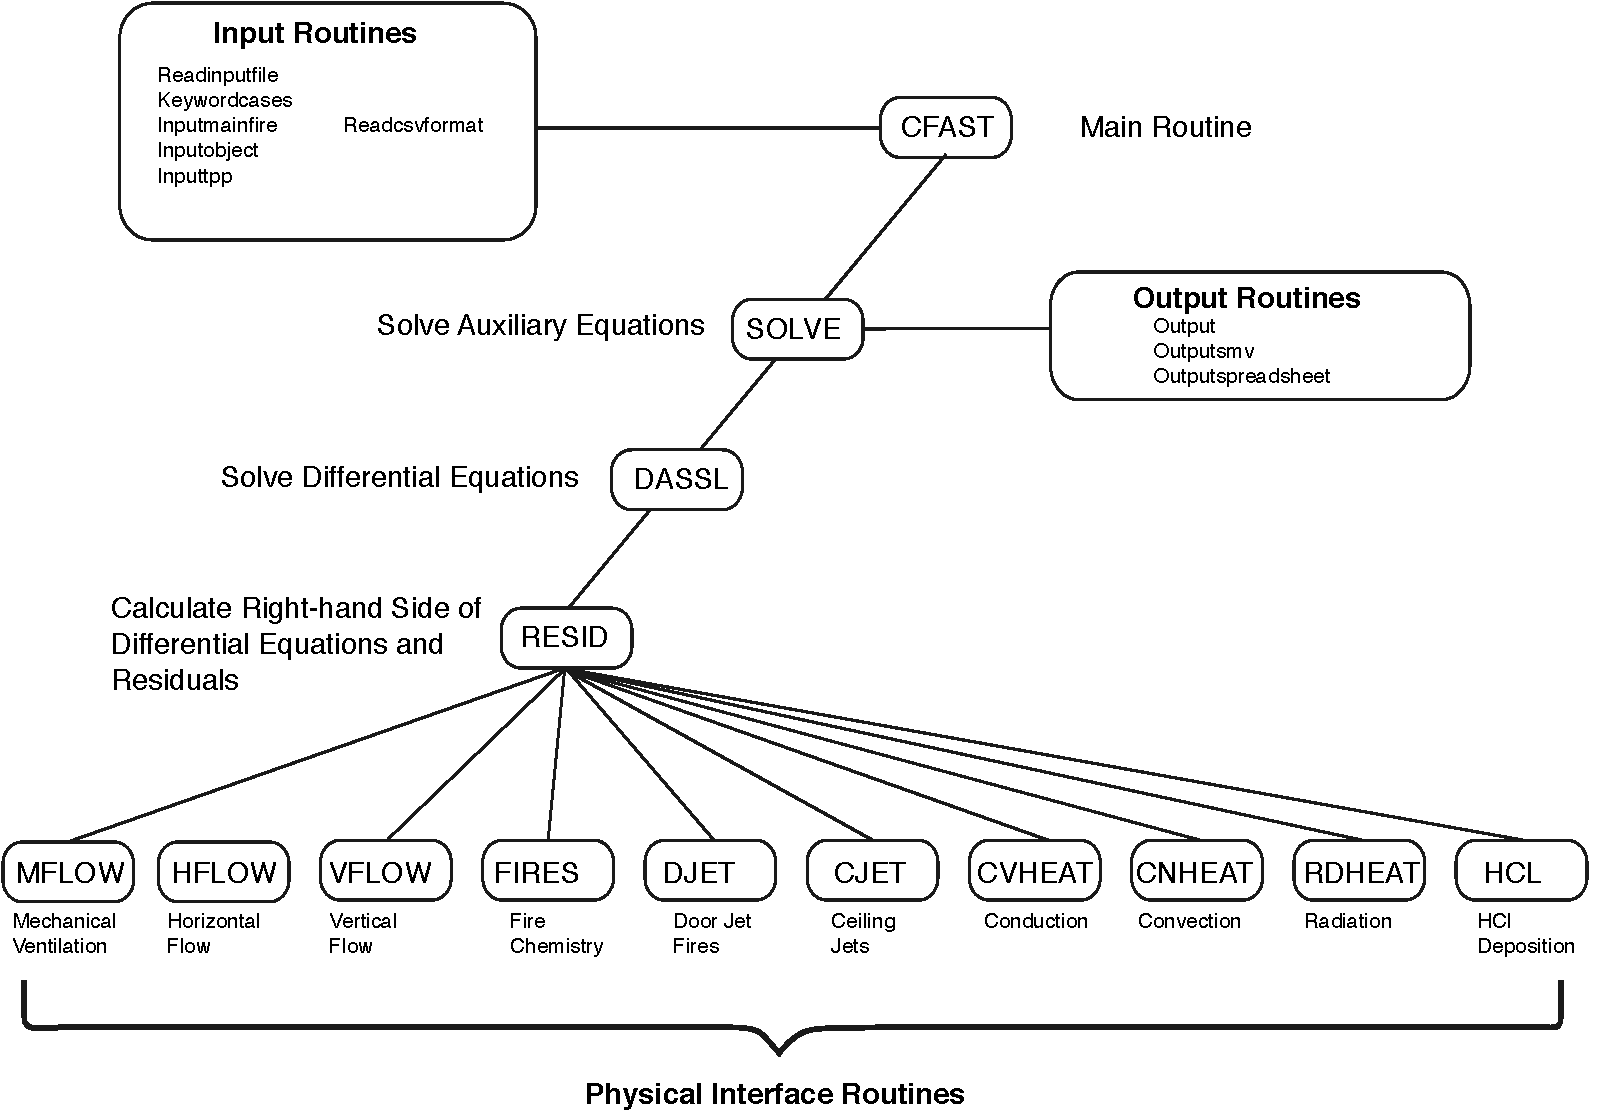
\includegraphics[width=6.4in]{FIGURES/Robustness/Structure}\\
\end{center}
\caption{Subroutine structure for the CFAST model.}
 \label{fig:Subroutines}
\end{figure}

The routines SOLVE, RESID and DASSL are the key to understanding how the physical 
equations are solved.  SOLVE is the control program that oversees the general solution of the 
problem.  It invokes the differential equation solver DASSL \cite{DASSL} which in turn calls RESID to 
solve the transport equations.  Given a solution at time $t$, what is the solution at time t plus a 
small increment of time, $\Delta t$, (where the time increment is determined dynamically by the 
program to insure convergence of the solution at $t + \Delta t$)?  The differential equations are of the 
form 

\be
\frac{dy}{dt} = f(y,t) \; , \; y(t_0) = y_0
\label{eq:basicsolution}
\ee
where $y$ is a vector representing pressure, layer height, mass and such, and $f$ is a vector function
that represents changes in these values with respect to time.  The term $y_0$ is an initial condition at 
the initial time $t_0$ .  The subroutine RESID computes the right hand side of eq (\ref{eq:basicsoultion}) and returns a set of residuals of that calculation to be compared to the values expected by DASSL.  DASSL then checks for convergence.  Once DASSL reaches an error limit (defined as convergence of 
the equations) for the solution at $t + \Delta t$,  SOLVE then advances the solution of species concentra- 
tion, wall temperature profiles, and mechanical ventilation for the same time interval. 
Note that there are several distinct time scales that are involved in the solution of this type of 
problem.  The fastest will be chemical kinetics.  We avoid that scale by assuming that the 
chemistry is infinitely fast.  The next larger time scale is that associated with the flow field. 
These are the equations which are cast into the form of ordinary differential equations.  Then 
there is the time scale for mechanical ventilation, and finally, heat conduction through objects. 
Chemical kinetic times are typically on the order of milliseconds.  The transport time scale are 
on the order of 0.1 s.  The mechanical ventilation and conduction time scales are typically 
several seconds, or even longer.  The time step is dynamically adjusted to a value appropriate for 
the solution of the currently defined equation set.  In addition to allowing a more correct solution 
to the pressure equation, very large time steps are possible if the problem being solved 
approaches steady-state.

\section{Code Checking}

There are two means to automate checking the correctness of the language used by a numerical 
model. The first is the use of standard methods for checking the structure and interface. 
Programs such as Flint and Lint are standard tools to do such checking. They are applied to the 
whole model. There are three aspects of the model checked by this procedure: correctness of the 
interface, undefined or incorrectly defined (or used) variables and constants, and completeness 
of loops and threads. It does not check for the correctness of the numerical use of constants or 
variables only that they are used correctly in a syntactical sense. Lint is part of most C language 
distributions of Unix. Flint is the equivalent for the FORTRAN language. Though it is not 
usually included with FORTRAN distributions Flint is generally available \footnote{Cleanscape Software, 445 Sherman Ave, Ste. Q, Palo Alto, CA 94306}. Both have been used with CFAST. 

The second is to use a variety of computer platforms to compile and run the code. Since 
FORTRAN and C are implemented differently for various computers, this represents both a 
numerical check as well as a syntactic check. CFAST has been compiled for the Sun (Solaris), 
SGI (Irix), the windows-based PCs (Lahey, Digital, and Intel FORTRAN), and the Concurrent 
Computer platforms. Within the precision afforded by the various hardware implementations, the 
answers are identical \footnote{Typically one part in 10\superscript{-6}, which is the error limit used for DASSL.}.

\section{Numerical Tests}

There are two components to testing the numerical solutions of CFAST.  First, the DASSL 
solver is well tested for a wide variety of differential equations, and is widely used and accepted 
\cite{DASSL}. Also, the radiation and conduction routines are tested with known solutions. These are not 
analytical tests, but physical limits, such as an object immersed in a fluid of constant 
temperature, to which the temperature must equilibrate. The solver(s) must show that the 
differential equations asymptotically converge to these answers. 

The second is to insure that the coupling between algorithms and the solver is correct. Most 
errors are avoided because of the structure discussed in section \ref{sec:Subroutines}. The error due to the numerical solution is far less than that associated with the model assumptions. Two examples of 
this are the coupling of mechanical ventilation with buoyant flow, and the Nusselt number 
assumption for boundary layer convection. For the former, the coupling of a network of 
incompressible flow with an ODE for compressible flow has to deal with disparate calculations 
of pressure. For the latter, a very small time step occurs when a floor is heated and the thermal 
wave reaches the far (unexposed) side. This is a limitation of the physical implementation of the 
heat flow algorithm (convection). The solver arrives at the correct solution, but the time step 
becomes very small in order to achieve this. 

Numerical error can be divided into three categories: roundoff, truncation and discretization 
error. Roundoff error occurs because computers represent real numbers using a finite number of 
digits. Truncation error occurs when an infinite process is replaced by a finite one. This can 
happen, for example, when an in finite series is truncated after a finite number of terms or when 
an iteration is terminated after a convergence criterion has been satisfied. Discretization error 
occurs when a continuous process such as a derivative is approximated by a discrete analog such 
as a divided difference. CFAST is designed to use 64-bit precision for real number calculations 
to minimize these effects. 

Implicit in solving the equations discussed in chapter \ref{sec:Theory_Chapter}, is that the solver will arrive at a solution.  Inherent in the DASSL solver are convergence criteria for the mass and energy balance within CFAST to insure mass and energy conservation within 1 part in 10\superscript{6}.  There are, however, limitations introduced by the algorithmic realization of physical models, that can produce errors and instabilities. Using the example above, if a mechanical ventilation system injects or removes 
mass and enthalpy from a small duct, then there can be a stability issue with the layer interface 
bobbing up and down over the duct. These are annoyances to the user community and 
shortcomings of the implementation of algorithm rather than failure of the system model.

Problems of this sort are noted in the �frequently asked questions� on the CFAST web site 
(http://cfast.nist.gov).

\section{Comparison with Analytic Solutions}

There do not exist general analytic solutions for fire problems, even for the simplest cases. That 
is, there are no closed form solutions to this type of problem. However, it is possible to do two 
kinds of checking. The first type is discussed in the section on the theoretical basis of the model, 
for which individual algorithms are validated against experimental work. The second is simple 
experiments, especially for conduction and radiation, for which the results are asymptotic. For 
example, for a simple, single compartment test case with no fire, all temperatures should 
equilibrate asymptotically to a single value.  Such comparisons are common and not usually 
published.
\chapter{Sensitivity of the Model}

A sensitivity analysis considers the extent to which uncertainty in model inputs influences model 
output.  For a sensitivity analysis, this uncertainty includes not only that inherent in the input of 
data for specific scenarios by the model user, but also uncertainty in empirical data or numerical 
parameters in the model such as the time step size used by the model to obtain a solution. 

Among the purposes for conducting a sensitivity analysis are to determine 
\begin{itemize}
\item the important variables in the models, 
\item the computationally valid range of values for each input variable, and 
\item the sensitivity of output variables to variations in input data. 
\end{itemize}

Conducting a sensitivity analysis of a complex model is not a simple task and it will differ 
depending on the application. CFAST typically requires the user to provide numerous input 
parameters that describe the building geometry, compartment connections, construction 
materials, and description of one or more fires. 

Iman and Helton \cite{Iman:1988} studied the sensitivity of complex computer models developed to simulate the risk of severe nuclear accidents which may include fire and other risks. Consistent with the 
work of Iman and Helton \cite{Iman:1988}, ASTM E1355 \cite{ASTM:E1355} provides overall guidance on typical areas of evaluation of the sensitivity of deterministic fire models.  These areas may involve one or more of the following techniques: finite difference or direct analysis methods that provide an explicit solution of the sensitivity equations associated with the governing equations of the model, 
factorial design or Latin hypercube sampling studies that investigate the effect of varying the 
input parameters and consequential interactions between parameters that may be deemed 
important, and global or response surface methods that investigate the overall behavior of model 
outputs for a desired range of inputs. 

This chapter provides a review of the sensitivity studies that have been conducted using CFAST 
with an emphasis on uncertainty in the input. Other sensitivity investigations of CFAST are also 
available \cite{Peacock:1988a, Beard:1992, Notarianni:2000}. 

\section{Factorial Design Studies}

Khoudja [\cite{Khoudja:1988} has studied the sensitivity of an early version of the FAST [2] (predecessor to CFAST) model with a fractional factorial design involving two levels of 16 different input 
parameters. The statistical design, taken from the texts by Box and Hunter \cite{Box:1978}, and Daniel \cite{Daniel:1976} reduced the necessary model runs from more than 65 000 to 256 by studying the interactions of input parameters simultaneously. The choice of values for each input parameter represented a range for each parameter. The analysis of the FAST model showed sensitivity to heat loss to the compartment walls and to the number of compartments in the simulation. Without the inclusion 
of surface thermophysical properties, this model treats surfaces as adiabatic for conductive heat 
transfer. Thus, consistent sensitivity should be expected. Sensitivity to changes in thermal 
properties of the surfaces were not explored. 

Walker \cite{Walker:1997} discussed the uncertainties in components of zone models and showed how 
uncertainty within user-supplied data affects the results of calculations using CFAST as an 
example. The study systematically varied inputs related to the fire (heat release rate, heat of 
combustion, mass loss rate, radiative fraction, and species yields) and compartment geometry 
(vent size and ceiling height) ranging from  $\pm$ 1 \% to $\pm$ 20 \% of base values for a one- 
compartment scenario. Heat release rate and ceiling height are seen to be the dominant input 
variables in the simulations. Upper layer temperature changed $\pm$ 10 \% for a $\pm$ 10 \% change in 
heat release rate. Typical variation of $\pm$ 10 s in time to untenable conditions for a 20 \% variation 
in the inputs was noted for the scenarios studied. 

Peacock et al. \cite{Peacock:1988a} studied the sensitivity of CFAST for a range of input parameters. They used simple factorial designs for model inputs deemed important to investigate local behavior of 
important model outputs along with response surface methods to evaluate overall model 
behavior. Results of the parametric investigations are discussed below and the application of 
response surface methods is summarized in section 5.2. Both are discussed in more detail in 
reference \cite{Peacock:1988a}.

\subsection{Model Inputs and Outputs}

Most studies of modeling related to fire hazard and fire reconstruction present a consistent set of 
variables of interest to the model user \cite{Emmons:1988, Duong:1990, Beard:1992, NRCNUREG1824Overview} : upper and lower gas layer temperatures, gas species concentrations, and layer interface position. Other variables of interest include 

\begin{itemize}
\item mass pyrolysis and heat release rate, 
\item room pressure, and 
\item vent flow. 
\end{itemize}

Although there are certainly other comparisons of interest, these will provide evidence of the 
sensitivity of the model to most model inputs.  Tables 4 and 5 show typical inputs and outputs 
for the CFAST model.

\begin{table}
\begin{center}
\caption{Typical Inputs for a Two-Zone Fire Model}
\label{tab:Two_Zone_Inputs}
\begin{tabular}{| c | c | c | c | c | c | c | c |}
\hline
\multirow{2}{*}{Surface} & $b_1$ & $b_2$ & $b_3$ & $b_4$ & $b_5$ & $b_6$ & $b_7$ \\
 & (m) & (m\superscript{3}/kg) & (s\superscript{-1}) & (J/g mol) & (m\superscript{3}/kg)\superscript{$b_7 - b_6$} & (note a) & (note b) \\ 
 \hline
 Painted Gypsum & 0.0063 & 191.8 & 0.0587 & 7476 & 193 & 1.021 & 0.431 \\ \hline
 PMMA & $9.6 x 10^{-5}$ & 0.0137 & 0.0205 & 7476 & 29 & 1.0 & 0.431 \\ \hline
 Ceiling Tile & $4.0 x 10^{-3}$ & 0.0548 & 0.123 & 7476 & 30\superscript{a} & 1.0 & 0.431 \\ \hline
 Cement Block & $1.8 x 10^{-2}$ & 5.48 & 0.497 & 7476 & 30\superscript{a} & 1.0 & 0.431 \\  \hline
 Calcium Silicate Board & $1.9 x 10^{-2}$ & 0.137 & 0.030 & 7476 & 30\superscript{a} & 1.0 & 0.431 \\  \hline
\end{tabular}
\end{center}
a - very approximate value, insufficient data for high confidence value

b - non-dimensional
\end{table}

\begin{table}
\begin{center}
\caption{Typical Outputs for a Two-Zone Fire Model}
\label{tab:Two_Zone_Outputs}
\begin{tabular}{| c | c | c | c | c | c | c | c |}
\hline
\multirow{2}{*}{Surface} & $b_1$ & $b_2$ & $b_3$ & $b_4$ & $b_5$ & $b_6$ & $b_7$ \\
 & (m) & (m\superscript{3}/kg) & (s\superscript{-1}) & (J/g mol) & (m\superscript{3}/kg)\superscript{$b_7 - b_6$} & (note a) & (note b) \\ 
 \hline
 Painted Gypsum & 0.0063 & 191.8 & 0.0587 & 7476 & 193 & 1.021 & 0.431 \\ \hline
 PMMA & $9.6 x 10^{-5}$ & 0.0137 & 0.0205 & 7476 & 29 & 1.0 & 0.431 \\ \hline
 Ceiling Tile & $4.0 x 10^{-3}$ & 0.0548 & 0.123 & 7476 & 30\superscript{a} & 1.0 & 0.431 \\ \hline
 Cement Block & $1.8 x 10^{-2}$ & 5.48 & 0.497 & 7476 & 30\superscript{a} & 1.0 & 0.431 \\  \hline
 Calcium Silicate Board & $1.9 x 10^{-2}$ & 0.137 & 0.030 & 7476 & 30\superscript{a} & 1.0 & 0.431 \\  \hline
\end{tabular}
\end{center}
a - very approximate value, insufficient data for high confidence value

b - non-dimensional
\end{table}

Consider the following fire scenario: The building geometry (figure \ref{fig:Sensitivity_BaseCase}) includes four rooms on two floors with horizontal, vertical, and mechanical vents connecting the rooms and venting to the outdoors. The fire source in one of the rooms on the lower floor is a medium growth rate t-squared fire \cite{NFPA72:2003} chosen to simulate a mattress fire \cite{Babrauskas:1985}.

\begin{figure}[t]
\begin{center}
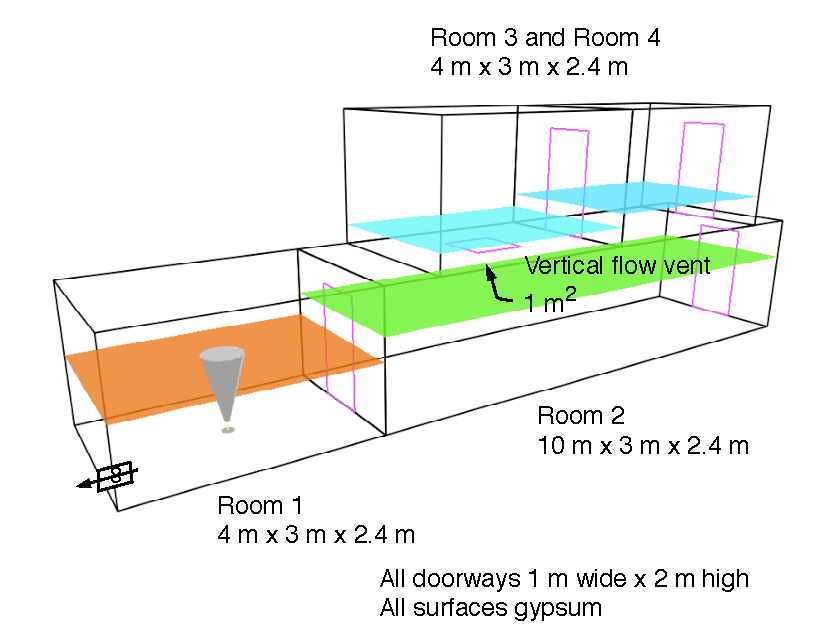
\includegraphics[width=4.5in]{FIGURES/Sensitivity/SensitivitySample}\\
\end{center}
\caption{Building Geometry for base case scenario.}
 \label{fig:Sensitivity_BaseCase}
\end{figure}

\chapter{Survey of Past Validation Work} \label{sec:validationsummary}

CFAST has been subjected to extensive validation studies by NIST and others.  There are two ways of comparing predictive capability with actual events. The first is simply graphing the time series curves of model results with measured values of variables such as temperature. Another approach is to consider the time to critical conditions such as flashover. Making such direct comparisons between theory and experiment provides a sense of whether predictions are reasonable. This chapter provides a review of CFAST validation efforts by NIST and others to better understand the quality of the predictions by the model.

Some of the work has been  performed at NIST, some by its grantees and some by engineering firms using the model.  Because each organization has its  own reasons for  validating the model, the  referenced papers and reports do not follow any particular guidelines. Some of the works only provide  a qualitative assessment  of the model,  concluding that the  model  agreement with  a  particular  experiment  is ``good''  or ``reasonable.'' Sometimes, the conclusion is that the model works well in certain cases, not as well in others. These studies are included in the survey because the references  are useful to other model users who may have a similar application  and are interested in qualitative assessment. It is important to note  that some of the papers point out flaws in early releases of CFAST that have been corrected or improved in more recent  releases. Some of  the issues raised, however,  are still subjects of  active research. Continued updates for CFAST  are greatly influenced  by   the  feedback   provided  by  users,   often  through publication of validation efforts.


\section{Comparisons with Full-Scale Tests Conducted Specifically for the Chosen Evaluation}

Several studies have been conducted specifically to validate the use of CFAST in building performance design. Dembsey   \cite{Valid:Dempsey} used CFAST version 3.1 to predict the ceiling jet temperatures, surface heat fluxes and heat transfer coefficients for twenty compartment fire experiments in a compartment that is similar in size, geometry, and construction to the standard fire test compartment specified in the Uniform Building Code \cite{UBC}\footnote{The 1997 Uniform Building Code has been superceded by the International Building Code, 2003 Edition, International Code Council, Country Club Hills, Illinois.}. Results from 330 kW, 630 kW, and 980 kW fires were used. In general, CFAST made predictions which were higher than the experimental results. In these cases, the temperature prediction is typically 20 \% to 30 \% higher than measured values. Much of this can be attributed to not knowing the species production (soot) and relative absorption of radiation by the gas layers which highlights the importance of scenario specification. This is the most common cause of  �over prediction� of temperature by CFAST. A secondary source of discrepancy is correcting for radiation from thermocouple beads. The authors provide for this correction, but the corrections cited are not as large as has been reported in other fire experiments \cite{Valid:Pitts}.

He et al. \cite{Valid:He} describe a series of full-scale fire experiments that were designed to investigate the validity of two zone models including CFAST version 3.1. The experiments, involving steady state burning rates and a number of ventilation conditions, were conducted in a four-story building. Temperature, pressure, flow velocity, smoke density and species concentrations were measured in various parts of the building. The stack effect and its influence on temperature distribution in a stair shaft were observed. Comparisons were then made between the experimental results and the model predictions. Early in the fire there is a few percent difference\footnote{Unless otherwise noted, percent differences are defined as (model-experiment)/experiment x100.} between the predictions and measurements; beyond 10 min, there are significant variations. Both the experiment and the model are internally consistent; that is, higher flow leads to a higher interface height (figure 13 in the paper). Once again, the difference is about 25 \%. The authors discuss the effect of fuel composition and correction for radiation from thermocouple beads but did not draw firm conclusions based on their measurements of fuel products.

A series of experimental results for flaming fires, obtained using realistic fires in a prototype apartment building were performed by Luo et al. \cite{Valid:Luo}. Fuel configurations in the fire test included a horizontal plain polyurethane slab, mock-up chair (polyurethane slabs plus a cotton linen cover), and a commercial chair. CFAST version 3.1 typically over-predicted upper layer temperatures by 10 \% to 50 \% depending on the test conditions and measurement location in that test. The predicted and experimental time dependent upper layer temperatures were similar in shape. The time to obtain peak upper layer temperatures was typically predicted to within 15 \% of the experimental measurements. The authors concluded that CFAST was conservative in terms of life safety calculations.

In order to optimize fire service training facilities, the best use of resources is imperative. The work reported by Poole et al. \cite{Valid:Poole} represents one aspect of a cooperative project between the city of Kitchener Fire Department (Canada) and the University of Waterloo aimed at developing design criteria for the construction of a fire fighter training facility. One particular criterion is that realistic training with respect to temperature, heat release and stratification be provided in such a facility. The purpose of this paper was to compare existing analytical heat release and upper and lower gas temperature rise correlations and models with data from actual structures which were instrumented and burned in collaboration with the Kitchener Fire Department. According to the authors, the CFAST model was used `successfully' to predict these conditions and will be used in future design of such facilities.

A report by Bailey et al. \cite{Valid:Bailey_Shadwell} compares predictions by CFAST version 3.1 to data from real scale fire tests conducted onboard ex-USS SHADWELL, the {Navy's} R\&D damage control platform. The phenomenon of particular interest in this validation series was the conduction of heat in the vertical direction through compartment ceilings and floors. As part of this work, Bailey et al. \cite{Valid:Bailey_Vertical_Heat} compared CFAST temperature predictions on the unexposed walls of large metal boxes, driven by steady state fires. This tested the model�s prediction of radiation and conduction in both the vertical and horizontal directions. Indirectly it quantifies the quality of the conduction/convection/radiation models. The model and experiment compared well within measurement error bounds of each. The comparison was particularly good for measurements in the fire compartment as well as for the compartment and deck directly above it, with predictions typically agreeing with experiments within measurement uncertainty. The model under-predicted the temperatures of the compartments and decks not directly adjacent to the fire compartment early in the tests. Most of the error arose due to uncertainty in modeling the details of the experiment. The size of the vent openings between decks and to the outside must be included, but these were not always known. Cracks formed in the deck between the fire compartment and the compartment above due to the intense fire in the room of origin, but a time dependent record was not kept. The total size of the openings to the outside of warped doors in both compartments was not recorded. As can be seen in figures 7 and 8 of reference \cite{Valid:Bailey_Shadwell}, the steady state predictions are identical (within error bounds of the experiment and prediction). The largest error is after ignition (uncertainty in the initial fire) and during development of the cracks between the compartments. While this does not affect the agreement in the room of origin, it does lead to an uncertainty of about 30 \% in the adjacent compartment.

\section{Comparisons with Previously Published Test Data}

A number of researchers have studied the level of agreement between computer fire models and
real-scale fires. These comparisons fall into two broad categories: fire reconstruction and
comparison with laboratory experiments. Both categories provide a level of verification for the
models used. Fire reconstruction, although often more qualitative, provides a higher degree of
confidence for the user when the models successfully simulate real-life conditions. Comparisons
with laboratory experiments, however, can yield detailed comparisons that can point out
weaknesses in the individual phenomena included in the models.

Deal \cite{Valid:Deal} reviewed four computer fire models (CCFM \cite{Models:CCFM}, FIRST \cite{Models:FIRST}, FPETOOL \cite{Models:FPETool} and FAST \cite{Models:FAST} version 18.5 (the immediate predecessor to CFAST)) to ascertain the relative performance of the models in simulating fire experiments in a small room (about 12 m$^3$ in volume) in which the vent and fuel effects were varied. Peak fire size in the experiments ranged up to 800 kW. According to the author, all the models simulated the experimental conditions including temperature, species generation, and vent flows `quite satisfactorily.' With a variety of conditions, including narrow and normal vent widths, plastic and wood fuels, and flashover and sub-flashover fire temperatures, competence of the models at these room geometries was `demonstrated.'

NIST has studied the predictive capability of CFAST in detail for several scenarios where 
experimental data were available. Peacock et al. \cite{Peacock:1993d} compared the performance of the CFAST model with experimental measurements for the variables presented above. Using a range of 
laboratory tests, they presented comparisons of peak values, average values, and overall curve 
shape for a number of variables of interest to model users. A total of five different real-scale fire 
tests were selected for the comparisons to represent a range of challenges for the CFAST model. 
Details of the experimental measurements and procedure for model calculations are available in 
the original paper \cite{Peacock:1993d}. Typical agreement between model predictions and experimental values ranged from about 2 \% to 25 \%. Careful specification of a simulation and building leakage were seen as important factors in assuring an accurate prediction.

\subsection{NIST/NRC Verification and Validation}

The U.S. Nuclear Regulatory Commission performed an extensive verification and validation 
of several fire models commonly used in nuclear power plant applications \cite{NRCNUREG1824_CFAST}. These models included simple spreadsheet calculations, zone models (including CFAST), and CFD models. The results of this study are presented in the form of relative differences between fire model predictions and experimental data for fire modeling attributes such as plume temperature that are important to NPP fire modeling applications. While the relative differences sometimes show agreement, they also show both under-prediction and over-prediction in some circumstances. These relative differences are affected by the capabilities of the models, the availability of accurate applicable experimental data, and the experimental uncertainty of these data. The 
two-zone models performed well when compared with the experiments considered. Evaluation 
of the two-zone models showed that the models simulated the experimental results within 
experimental uncertainty for most of the parameters of interest The reason for this may be that 
the relatively simple experimental configurations selected for this study conform well to the 
simple two-layer assumption that is the basis of these models. However, users must remain 
cautious when applying these models to more complex scenarios, or when predicting certain 
phenomena, like heat fluxes. The results and comparisons included the the NRC study are 
included in the CFAST Software Development and Experimental Evaluation Guide for the current version of CFAST \cite{CFAST_Valid_Guide_6}.

\subsection{Fire Plumes}

Davis compared predictions by CFAST version 5 (and other models) for high ceiling spaces \cite{Valid:Davis_Plumes}. In this paper, the predictive capability of two algorithms designed to calculate plume centerline temperature and maximum ceiling jet temperature in the presence of a hot upper layer were compared to measurements from experiments and to predictions using CFAST�s ceiling jet algorithm. The experiments included ceiling heights of 0.58 m to 22 m and heat release rates of 0.62 kW to 33 MW. When compared to the experimental results CFAST�s ceiling jet algorithm tended to over-predict the upper layer temperature by 20 \%. With proper adjustment for radiation effects in the thermocouple measurements, some of this difference disappears. The effect of entrainment of the upper layer gases was identified for improvement.

\subsection{Multiple Compartments}
\label{secMultipleCompartments}

Jones and Peacock \cite{Valid:Jones} presented a limited set of comparisons between the FAST model (version 18.5) and a multi-room fire test. The experiment involved a constant fire of about 100 kW in a three-compartment configuration of about 100 m$^3$. They observed that the model predicted an upper layer temperature that was too high by about 20 \% with satisfactory prediction of the layer interface position. These observations were made before the work of Pitts et al. \cite{Valid:Pitts} showed that the thermocouple measurements need to be corrected for radiation effects. Convective heating and plume entrainment were seen to limit the accuracy of the predictions. A comparison of predicted and measured pressures in the rooms showed within 20 \%. Since pressure is the driving force for flow between compartments, this agreement was seen as important.

Levine and Nelson \cite{Valid:Levine} used a combination of full-scale fire testing and modeling to simulate a fire in a residence. The 1987 fire in a first-floor kitchen resulted in the deaths of three persons in an upstairs bedroom, one with a reported blood carboxyhemoglobin content of 91 \%. Considerable physical evidence remained. The fire was successfully simulated at full scale in a fully-instrumented seven-room two-story test structure. The data collected during the test have been used to test the predictive abilities of two multiroom computer fire models: FAST and HARVARD VI. A coherent ceiling layer flow occurred during the full-scale test and quickly carried high concentrations of carbon monoxide to remote compartments. Such flow is not directly accounted for in either computer code. However, both codes predicted the carbon monoxide buildup in the room most remote from the fire. Prediction of the pre-flashover temperature rise was also `good' according to the authors. Prediction of temperatures after flashover that occurred in the room of fire origin was seen as `less good.' Other predictions of conditions throughout the seven test rooms varied from `good approximations' to `significant deviations' from test data. Some of these deviations are believed to be due to combustion chemistry in the not upper layer not considered in detail in either of the two models.

\subsection{Large Compartments}

Duong \cite{Valid:Duong} studied the predictions of several computer fire models (CCFM, FAST, FIRST, and BRI \cite{Models:BRI}), comparing the models with one another and with large fires (4 MW to 36 MW) in an aircraft hanger (60 000 m$^3$). For the 4 MW fire size, he concluded that all the models are `reasonably accurate.' At 36 MW, however, `none of the models did well.' Limitations of the heat conduction and plume entrainment algorithms were thought to account for some of the inaccuracies.

\subsection{Prediction of Flashover}

A chaotic event that can be predicted by mathematical modeling is that of flashover. Flashover is
the common term used for the transition a fire makes from a few objects pyrolyzing to full room
involvement. It is of interest to the fire service because of the danger to fire fighters and to
building designers because of life safety and the attendant impact on occupants. Several papers
have looked at the capability of CFAST to predict the conditions under which flashover can
occur.

Chow \cite{Valid:Chow_Flashover} concluded that FAST correctly predicted the onset of flashover if the appropriate criteria were used. The criteria were gas temperature near the ceiling, heat flux at the floor level and flames coming out of the openings. This analysis was based on a series of compartment
fires.

A paper by Luo et al. \cite{Valid:Luo_Flashover} presents a comparison of the results from CFAST version 3 against a comprehensive set of data obtained from one flashover fire experiment. The experimental results were obtained from a full-scale prototype apartment building under flashover conditions. Three polyurethane mattresses were used as fuel. It was found that the predicted temperatures from the CFAST fire model agreed well with the experimental results in most areas, once radiation corrections are applied to the thermocouple data.

Collier \cite{Valid:Collier} makes an attempt to quantify the fire hazards associated with a typical New
Zealand dwelling with a series of experiments. These tests, done in a three-bedroom dwelling,
included both non-flashover and flashover fires. The predictions by CFAST version 2 were seen by the author as consistent with the experiments within the uncertainty of each.

Post-flashover fires in shipboard spaces have a pronounced effects on adjacent spaces due to
highly conductive boundaries. CFAST (version 3.1) predictions for the gas temperature and the
cold wall temperature were compared with shipboard fires \cite{Valid:White}. The comparisons between the model and experimental data show `conservative predictions' according to the authors. The authors attribute this to an overestimation of the average hot wall temperature and an underestimation of external convective losses due to wind effects.

Finally, a comparison of CFAST with a number of simple correlations was used by
Peacock and Babrauskas \cite{Valid:Peacock_Flashover_1,Valid:Peacock_Flashover_2} to simulate a range of geometries and fire conditions to predict the development of the fire up to the point of flashover. The simulations represent a range of compartment sizes and ceiling heights. Both the correlations and CFAST predictions were seen to provide a lower bound to observed occurrence of flashover. For very small or very large compartment openings, the differences between the correlations, experimental data, and CFAST predictions was more pronounced.

The important test of all these prediction methods is in the comparison of the predictions with
actual fire observations. Figure \ref{figValidFlashover} (reference \cite{Valid:Peacock_Flashover_2}) presents estimates of the energy required to achieve flashover for a range of room and vent sizes. This figure is an extension of the earlier work of Babrauskas  \cite{Valid:Babrauskas_Flashover} and includes additional experimental measurements from a variety of sources, most notably the work of Deal and Beyler \cite{Valid:DealandBeyler}. For a number of the experimental observations, values are included that were not 
explicitly identi�ed as being a minimum value at flashover. In addition, figure \ref{figValidFlashover} includes predictions from the CFAST model (version 5).

\begin{figure}{t}
\begin{center}
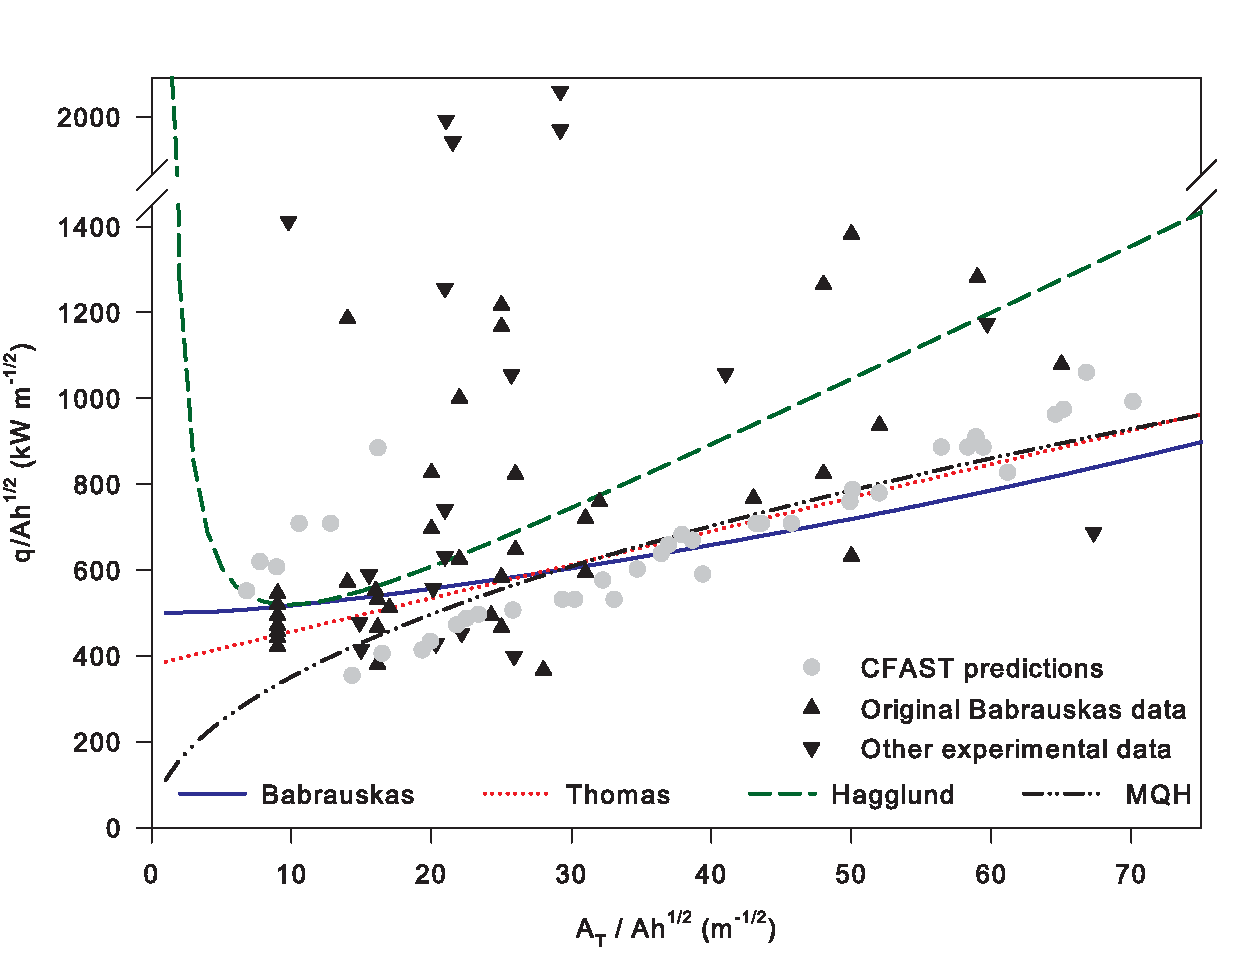
\includegraphics[width=4.5in]{FIGURES/Validation/flashover}\\
\end{center}
\caption{Comparison of correlations, CFAST predictions, and experimental data for the prediction of flashover in a compartment fire.}
 \label{figValidFlashover}
\end{figure}

As with some of the experimental data defining flashover as an upper layer temperature reaching
600 $^{\circ}$C, many experimental measures were reported as peak values rather than minimum values necessary to achieve flashover. Thus, ideally all the predictions should provide a lower bound
for the experimental data. Indeed, this is consistent with the graph � the vast majority of the
experimental observations lie above the correlations and model predictions. For a considerable
range in the ratio \asqh, the correlations of Babrauskas \cite{Valid:Babrauskas_Flashover} Thomas \cite{Thomas:1981fk}, and the MQH correlation of McCaffrey et al. \cite{McCaffrey:1981uq} provide similar estimates of the minimum energy required to produce flashover. The estimates of H\"{a}gglund \cite{Hagglund:1980} yields somewhat higher estimates for values of \asqh  \, greater than 20 m$^{-1/2}$.

The results from the CFAST model for this single compartment scenario provide similar results
to the experiments and the correlations for most of the range of \asqh. For small values of \asqh, the CFAST values rise somewhat above the values from the correlations. These small values of \asqh \, result from either very small compartments (small $A_T$) or very large openings (large \asqh), both of which stretch the limits of the assumptions inherent in the model. For very small compartments, radiation from the fire to the compartment surfaces becomes more important, enhancing the conductive heat losses through the walls. However, the basic two-zone assumption may break down as the room becomes very small. For very large openings, the calculation of vent flow via an orifice flow coefficient approach is likely inaccurate. Indeed, for such openings, this limitation has been observed experimentally \cite{Valid:Babrauskas_Flashover}. The estimates are close to the range of uncertainty shown by the correlations which also diverge at very small values of \asqh.

Perhaps most significant in these comparisons is that all the simple correlations provide estimates similar to the CFAST model and all the models are consistent with a wide range of experimental data. For this simple scenario, little is gained with the use of the more complex models. For more complicated scenarios, the comparison may not be as simple.

\section {Comparison with Documented Fire Experience}

There are numerous cases of CFAST being used to adjudicate legal disputes. Since these are discussed in courts of law, there is a great deal of scrutiny of the modeling, assumptions, and results. Most of these simulations and comparisons are not available in the public literature. A few of the cases which are available are discussed below. The metric for how well the model performed is its ability to reproduce the time-line as observed by witnesses and the death of occupants or the destruction of property as was used in evidence in legal proceedings.

As mentioned in section \ref{secMultipleCompartments}, Levine and Nelson describe the use of FAST for understanding the deaths of two adults in a residence in Sharon, Pennsylvania in 1987 \cite{Valid:Levine}. The paper compared the evidence of the actual fire, a full scale mockup done at NIST and the results from FAST (version 18) \cite{Jones:1985} and Harvard VI \cite{Rockett:1985}. The most notable shortcoming of the models was the lower than actual temperatures in the bedrooms, caused by loss of heat through the fire barriers. This led to the improvement in CFAST in the mid-90s to couple compartments together so that both horizontal and vertical heat transfer can occur to adjacent compartments.

Bukowski used CFAST version 3.1 to analyze a fire in New York City \cite{Bukowski:1996} in 1994 which resulted in the death of three fire fighters. The CFAST model was able to reproduce the observed conditions and supported the theory as to how the fire began and the cause of death of the three fire fighters.

Chow describes the use and comparison of CFAST simulations with a 1996 high rise building fire in Hong Kong \cite{Chow:1996}. CFAST simulations were performed to help understand the probable fire environment under different conditions. Three simulations were performed to study the consequences of a fire starting in the lift shaft. Smoke flow in the simulations qualitatively matched those observed during the incident.

In the early morning hours of March 25,1990 a tragic fire took the lives of 87 persons at a neighborhood club in the Bronx, New York \cite{Bukowski:1992}. The New York City Fire Department requested the assistance of the NIST Center for Fire Research (CFR) in understanding the factors which contributed to this high death toll and to develop a strategy that might reduce the risk of a similar occurrence in the many similar clubs operating in the city. The simulation showed the potential for development of untenable conditions within the club and particularly in the single exit stairway.

\section{Comparison with Experiments Which Cover Special Situations}

There are several sets of comparisons used in the development of the model or specific
applications beyond those discussed more generally above.

\subsection{Nuclear Facilities}

Floyd validated CFAST version 3.1 by comparing the modeling results with measurements from fire tests at
the Heiss-Dampf Reaktor (HDR) facility \cite{Floyd:2002}. The structure was originally the containment
building for a nuclear power reactor in Germany. The cylindrical structure was 20 m in diameter
and 50 m in height topped by a hemispherical dome 10 m in radius. The building was divided
into eight levels. The total volume of the building was approximately 11 000 m$^3$. From 1984 to
1991, four fire test series were performed within the HDR facility. The T51 test series consisted
of 11 propane gas tests and three wood crib tests. To avoid permanent damage to the test facility,
a special set of test rooms were constructed, consisting of a fire room with a narrow door, a long
corridor wrapping around the reactor vessel shield wall, and a curtained area centered beneath a
maintenance hatch. The fire room walls were lined with fire brick. The doorway and corridor
walls had the same construction as the test chamber. Six gas burners were mounted in the fire
room. The fuel source was propane gas mixed with 10 \% air fed at a constant rate to one of the
six burners.

In general, the comparison between CFAST and the HDR results was seen as `good' by the author, with two exceptions. The first is the over estimate of the temperature of the upper layer, typically within about 15 \% of the experimental measurements. This is common and generally results from using too low a value for the production of soot, water (hydrogen) and carbon monoxide. The other exception consists of predictions in spaces where the zone model concept breaks down, for example in the stairways between levels. In this case, CFAST has to treat the space either in the filling mode (two layer approximation) or as a fully mixed zone (using the SHAFT option). Neither is quite correct, and in order to understand the condition in such spaces in detail (beyond the transfer of mass and energy), a more detailed CFD model must be used, for example, FDS \cite{FDS_Tech_Guide_5}.

The U.S. Nuclear Regulatory Commission performed an extensive verification and validation of several fire models commonly used in nuclear power plant applications \cite{NRCNUREG1824}.  These models included simple spreadsheet calculations, zone models (including CFAST \cite{NRCNUREG1824_CFAST}), and CFD models. The results of this study are presented in the form of relative differences between fire model predictions and experimental data for fire modeling attributes such as temperature or heat flux that are important to NPP fire modeling applications.  These relative differences are affected by the capabilities of the models, the availability of accurate applicable experimental data, and the experimental uncertainty of these data. Evaluation of the two-zone models showed that the models simulated the experimental results within experimental uncertainty  for many of the parameters of interest. The reason for this may be that the relatively simple experimental configurations selected for this study conform well to the simple two-layer assumption that is the basis of these models. 

While the relative differences sometimes show agreement for many parameters, they also show both under-prediction and over-prediction in some circumstances, most notably when conditions vary within a compartment or detailed local conditions are important to accurate prediction (for example, plume temperature or heat flux near to the fire source). The results and comparisons included the the NRC study are included in this report for the current version of CFAST.

\subsection{Small Scale Testing}

As an implementation of the zone model concept, CFAST is applicable to a wide range of scenarios. One end of this spectrum are small compartments, one to two meters on a side. Several research efforts have looked at small scale validation. There are three papers by Chow \cite{Lui:2003,Chow:1995,Chow:1992} which examine this issue. The first is the use of an electric heater with adjustable thermal power output was to verify temperature predictions by CFAST version 3.1. The second was closed chamber fires studied by burning four types of organic liquids, namely ethanol, N-heptane, and kerosene. The burning behavior of the liquids was observed, and the hot gas temperature measured. These behaviors along with the transient variations of the temperature were then compared with those predicted by the CFAST model. Finally, in another series of experiments, three zone models, one of which was CFAST, were evaluated experimentally using a small fire chamber. Once again, liquid fires were chosen for having better control on the mass loss rate. The results on the development of smoke layer and the hot gas temperature predicted by the three models were compared with those measured experimentally. According to Chow, `fairly good agreement' was found if the input parameters were carefully chosen.

\subsection{Unusual Geometry and Specific Algorithms}

A zone model is inherently a volume calculation. There is an assumption in the derivation of the equations that gas layers are strongly stratified. This allows for the usual interpretation that a volume can then be thought of as a rectangular parallelepiped, which allows the developers to express the volume in terms of a floor area and height of a compartment, saying simply that the height times the floor area is the volume. However, there are other geometries which can be adequately described by zone models. Tunnels, ships, and attics are the most common areas of application which fall outside of the usual scope.

\subsubsection{Railway and Vehicle Tunnels}

Altinakar et al. \cite{Altinakar:1997} used a \emph{modified version} of CFAST for predicting fire development and smoke propagation in vehicle or railroad tunnels. The two major modifications made to the model dealt with mixing between the upper and lower layers and friction losses along the tunnel. The model was tested by simulating several full-scale tests carried out at memorial Tunnel Ventilation Test Program in West Virginia, and the Offeneg Tunnel in Switzerland. His article compares simulated values of temperature, opacity and similar sensible quantities with measured values and discusses the limits of the applicability of zone models for simulating fire and smoke propagation in vehicle and railroad tunnels. 

Peacock et al. \cite{Peacock:2004} compared times to untenable conditions determined from tests in a
passenger rail car with those predicted by CFAST for the same car geometry and fire scenarios.
For a range of fire sizes and growth rates, they found agreement that averaged approximately
13 \%.

\subsubsection{Non-Uniform Compartments}

In January 1996, the U.S. Navy began testing how the CFAST model would perform when tasked with predicting shipboard fires. These conditions include mass transport through vertical vents (representing hatches and scuttles), energy transport via conduction through decks, improvement to the radiation transport sub-model, and geometry peculiar to combat ships. The purpose of this study was to identify CFAST limitations and develop methods for circumnavigating these problems \cite{Hoover:2001}. A retired ship representing the forward half of a {USS} Los Angeles class submarine was used during this test. Compartments in combat ships are not square in floor area, nor do they have parallel sides.

Application of CFAST to these scenarios required a direct integration of compartment cross-sectional area as a function of height to correctly interpret the layer interface position and provide correct predictions for flow through doors and windows (vertical vents). This required user specification of the area as a function of height (ROOMA and ROOMH inputs) to provide a description for the model to use. For most applications of CFAST, the effort required for the input outweighs any additional precision in the calculated results gained by use of the ROOMA and ROOMH inputs in the model.

\subsubsection{Long Corridors}

Prior to development of the corridor flow model, the implementation of flow in compartments assumed that smoke traveled instantly from one side of a compartment to another. The work of Bailey et al. \cite{Bailey:2002} provided the basis for the corridor flow model in CFAST. According to the author, it shows `good agreement' for the delay time calculated using CFAST version 5 and measured flow along high aspect ratio passageways.

\subsubsection{Mechanical Ventilation}

There have been two papers which have looked at the effectiveness of the mechanical ventilation system. The first considered a fire chamber of length 4.0 m, width 3.0 m and height 2.8 m with adjustable ventilation rates \cite{Chow:1995a}. Burning tests were carried out with wood cribs and methanol to study the preflashover stage of a compartmental fire and the effect of ventilation. The mass loss rate of fuel, temperature distribution of the compartment and the air intake rate were measured. The heat release rates of the fuel were calculated and the smoke temperature was used as a validation parameter. A scoring system was proposed to compare the results predicted by the three models. According to the author, CFAST does `particularly well,' though there are some differences which can be attributed to the zone model approach.

A second series of experiments by Luo \cite{Luo:1997} indicate that the CFAST model (version 3.1) generally over predicts the upper layer temperature in the burn room because the two-zone assumption is likely to
break down in the burn room. It was found that the room �averaged temperatures obtained from
CFAST were in `good overall agreement' with the experimental results. The discrepancies can be
attributed to the correction needed for thermocouple measurements. The CO concentration,
however, was inconsistent. CFAST tended to overestimate CO concentration when the air
handling system was in operation. This was seen due to inconsistencies in what is measured
(point measurements) and predicted (global measurements).

\subsubsection{Sprinkler Activation}


A suppression algorithm \cite{Madrzykowski:1992} was incorporated into CFAST. Chow \cite{Chow:1996a} evaluates the predictive capability for a sprinkler installed in an atrium roof. There were three main points being considered: the possibility of activating the sprinkler, thermal response, and water requirement. The zone model CFAST was used to analyze the possibility of activation of a sprinkler head. Results derived from CFAST were seen to be `accurate, that is, providing good agreement with experimental measurements.'

\subsubsection{t$^2$ Fires}

Matsuyama conducted a series of full-scale experiments \cite{Matsuyama:2000} using t$^2$ fires. Fire room and corridor smoke filling processes were measured. The size of the corridors and arrangements of smoke curtains were varied in several patterns. Comparisons were then made between the experimental results and those predicted by CFAST. The author concludes that while the model does a `good job' of predicting experimental results, there are systematic differences which could be reduced with some revision to zone model formulation to include the impact of smoke curtains.

\section{Summary}

How to best quantify the comparisons between model predictions and experiments is not obvious. The necessary and perceived level of agreement for any variable is dependent upon both the typical use of the variable in a given simulation, the nature of the experiment, and the context of the comparison in relation to other comparisons being made. For instance, the user may be interested in the time it takes to reach a certain temperature in the room, but have little or no interest in peak temperature for experiments that quickly reach a steady-state value. Insufficient experimental data and understanding of how to compare the numerous variables in a complex fire model prevent a complete validation of the model. 

A true validation of a model would involve proper statistical treatment of all the inputs and outputs of the model with appropriate experimental data to allow comparisons over the full range of the model. Thus, the comparisons of the differences between model predictions and experimental data discussed here are intentionally simple and vary from test to test and from variable to variable due to the changing nature of the tests and typical use of different variables. Table \ref{tab:Summary_Relative_Diffs} summarizes the Validation comparisons included for the current version of the model detailed in the Software Development and Experimental Evaluation Guide for CFAST \cite{CFAST_Valid_Guide_6}.

\begin{table}[h]
\begin{center}
\caption{Summary of Model Comparisons}
\label{tab:Summary_Relative_Diffs}
\vspace{0.1in}
\begin{tabular*}{1.0\textwidth}{@{\extracolsep{\fill}} | l | c | c | c | c |}
\hline
Quantity & Average & Median & Within & 90th \\
& Difference$^{a}$ &Difference$^b$ & Experimental & Percentile$^d$ \\
& & & Uncertainty$^c$ & \\
& (\%) & (\%) & (\%) & (\%) \\
\hline
HGL Temperature & 6 &  14 &  52 &  30  \\ \hline
HGL Depth & 3 & 15 & 40 & 28 \\ \hline
Ceiling Jet Temperature & 16 & 5 & 70 & 61 \\ \hline
Oxygen Concentration & -6 & 18 & 12 & 32 \\ \hline
Carbon Dioxide Concentration & -16 & 16 & 21 & 52 \\ \hline
Smoke Obscuration$^e$ & 272/22 & 227/18 & 0/82 & 499/40 \\ \hline
Pressure & 43 & 13 & 77 & 206$^f$ \\ \hline
Target Flux (Total) & -23 & 27 & 42 & 51 \\ \hline
Target Temperature & 0 & 18 & 38 & 34 \\ \hline
Surface Flux (Total) & 5 & 25 & 40 & 61 \\ \hline
Surface Temperature & 24 & 35 & 17 & 76 \\ \hline
\end{tabular*}  
\end{center}
a - average difference includes both the sign and magnitude of the relative differences in order to show any general trend to over- or under-prediction. \\
b - median difference is based only on the magnitude of the relative differences and ignores the sign of the relative differences so that values with opposing signs do not cancel and make the comparison appear closer than individual magnitudes would indicate. \\
c - the percentage of model predictions that are within experimental uncertainty. \\
d - 90 \% of the model predictions are within the stated percentage of experimental values. For reference, a difference of 100~\% is a factor of 2 larger or smaller than experimental values. \\
e - the first number is for the closed door NIST/NRC tests and the second number if for the open door NIST/NRC tests. \\
f - high magnitude of the 90th percentile value driven in large part by two tests where under-prediction was approximately 2 Pa.
\end{table}

CFAST predictions in this validation study were consistent with numerous earlier studies, which show that the use of the model is appropriate in a range of fire scenarios.  The CFAST model has been subjected to extensive evaluation studies by NIST and others.  Although differences between the model and the experiments were evident in these studies, most differences can be explained by limitations of the model as well as of the experiments.  Like all predictive models, the best predictions come with a clear understanding of the limitations of the model and the inputs provided to perform the calculations.


\chapter{Conclusion}

CFAST is a collection of data, computer programs, and documentation which are used to simulate the important time-dependent phenomena describing the character of a compartment fire. The major functions provided include calculation of the buoyancy-driven as well as forced transport of energy and mass through a series of specified compartments and connections (e.g., doors, windows, cracks, ducts), and the resulting temperatures, smoke optical densities, and gas concentrations after accounting for heat transfer to surfaces and dilution by mixing with clean air.

CFAST is a zone model. The basic assumption of all zone fire models is that each compartment can be divided into a small number of control volumes, each of which is internally uniform in temperature and composition. Beyond these basic assumptions, the model typically involves a mixture of established theory (e.g., conservation equations), empirical correlations where there are data but no theory (e.g., flow and entrainment coefficients), and approximations where there are neither (e.g., post-flashover combustion chemistry) or where their effect is considered secondary compared to the �cost� of inclusion (e.g., temperature dependent material properties)..

The predictive equations are based on the fundamental laws of conservation of mass and energy. Empirical correlations are employed to bridge gaps in existing knowledge. Since the necessary approximations required by operational practicality result in the introduction of uncertainties in the results, the user should understand the inherent assumptions and limitations of the programs, and use these programs judiciously - including sensitivity analyses for the ranges of values for key parameters in order to make estimates of these uncertainties.

As discussed in this report, the CFAST model has been subjected to extensive evaluation studies by NIST and others. Although differences between the model and the experiments were evident in these studies, most differences can be explained by limitations of the model as well as of the experiments. Like all predictive models, the best predictions come with a clear understanding of the limitations of the model and of the inputs provided to do the calculations.

CFAST has proven to be fast, robust and reliable. While the focus of the development of the model has been whole building simulations for assessing the effect of fire on a building environ- ment, principally to calculate threats to life safety of occupants and insults to the building structure, it has been used for a wide variety of building and fire scenarios. The simplest use has been to as- certain the sufficiency of an air handling system to extract smoke. The most complex has been an assessment of fire propagation in a high-rise complex. It is also widely used as the fire model in egress calculations and is described as the basis for hazard estimates in the Simulex \cite{Thompson:1996} and Exodus \cite{Gwynne:2000} egress models.

Because of the speed of the model, it is possible to do real parameter studies of the building environment. It is reasonable to do actual parameter studies including the tens of thousands of variations needed for a proper hazard and risk calculation. Even in those cases where more de- tailed predictions are needed (e.g., smoke detector and sprinkler head siting), CFAST provides the capability to scope the problem, in essence doing parameter studies to determine what specific scenario should be addressed by more detailed calculations.

\backmatter


\bibliography{../Bibliography/CFAST_refs}
\addcontentsline{toc}{chapter}{References}
\end{document}
